\onehalfspacing
\fancypagestyle{plain}{
\fancyhf{}
\rhead{\thepage}
\renewcommand{\headrulewidth}{0pt}
\renewcommand{\footrulewidth}{0pt}
}

\chapter{COMPRENSIÓN DEL PROBLEMA}

\section{Marco teórico}

El presente marco teórico establece las bases físicas y conceptuales que fundamentan el estudio y justifican la necesidad de una monitorización climática dinámica. Comprender el comportamiento de los sistemas solares frente a las fluctuaciones ambientales es indispensable para evaluar su rendimiento real y superar las limitaciones espaciales que presentan los métodos de medición estáticos convencionales.

\subsection{Fundamentos de la conversión fotovoltaica}
La tecnología fotovoltaica se fundamenta en la conversión directa de la luz solar en electricidad mediante el efecto fotoeléctrico, utilizando como componente central celdas solares de materiales semiconductores, típicamente silicio, estructuradas internamente con una unión P-N, la cual es una unión física de un material semiconductor con huecos positivos (P) y con electrones negativos (N). A nivel físico, la radiación está compuesta por fotones; si la energía de estos impactos supera la banda de energía del material, logran liberar electrones de su estructura atómica. El campo eléctrico intrínseco de la celda se encarga entonces de separar estos portadores de carga, generando un movimiento direccionado que conforma una corriente continua lista para su aprovechamiento, transformación o almacenamiento \citep{martinez2018estimation}.

En la práctica, el rendimiento de esta conversión fotovoltaica no es un valor ideal fijo, sino que fluctúa en función de las condiciones meteorológicas del entorno operativo. Para predecir la potencia efectiva del sistema, se emplea un modelo matemático de estimación. Esta fórmula ajusta la potencia nominal estandarizada de fábrica considerando la cantidad real de luz solar incidente y las pérdidas por estrés térmico:

\begin{equation}
    P_{A} = P_{0} \frac{G_{i}}{1000} C_{K}
\end{equation}

donde:
\begin{itemize}
    \item $P_{0}$: Potencia máxima de instalación en condiciones estándar (W).
    \item $G_{i}$: Irradiancia global en el plano de la instalación ($W/m^{2}$).
    \item $C_{K}$: Factor de ajuste de potencia nominal por temperatura. Sin unidades. Calculado a través de la ecuación (9).
\end{itemize}

Dado que las condiciones estándar de prueba asumen una temperatura operativa ideal de 25 °C en la celda, el factor $C_{K}$ modela el cambio en la eficiencia cuando el panel tiene una temperatura diferente. Se calcula mediante la siguiente relación:

\begin{equation}
    C_{K} = 1 + \gamma_{P} * (T_{m} - 25)
\end{equation}

donde:
\begin{itemize}
    \item $\gamma_{P}$: Coeficiente relativo de temperatura. Entregado por el fabricante (en $\%.^{\circ}C^{-1}$).
    \item $T_{m}$: Temperatura del panel solar (en $^{\circ}C$).
\end{itemize}

Una vez que el sistema fotovoltaico ha sido montado, recibe luz solar y genera energía eléctrica. La combinación de valores de voltaje y corriente que puede entregar un sistema fotovoltaico se muestra en una gráfica denominada curva corriente contra voltaje (I-V). La Fig. 1-2 muestra una gráfica genérica, en la que la línea roja representa la curva I-V y la línea azul la relación de potencia total generada contra voltaje. Para generar la mayor cantidad de energía eléctrica se debe mantener el punto de operación cerca al punto de máxima potencia (MPP). Este punto corresponde a una combinación de valores entre la corriente de cortocircuito ($I_{SC}$) y el voltaje de circuito abierto ($V_{OC}$).

\subsection{Impacto de las variables meteorológicas y pérdidas técnicas}

El rendimiento de los sistemas fotovoltaicos no depende únicamente de sus especificaciones de diseño o fabricación, sino que está condicionado por las variaciones ambientales del entorno en el que operan. Cada instalación posee condiciones climáticas únicas que presentan desafíos diferentes para maximizar la eficiencia energética y optimizar las labores de mantenimiento \citep{chicaiza2024}.


\subsubsection{\textbf{Radiación solar:}} Representa el recurso energético primario. La radiación solar es directamente proporcional a la corriente generada por el panel fotovoltaico. Por lo tanto, cuando la irradiancia sube, la corriente de cortocircuito y la potencia máxima de salida del panel se incrementan \citep{Gonzalez2019Behavioral}. En la Figura \ref{fig:CurvasElectricasIrrTemp} (izquierda), se observa que, para un aumento de 600 a 1000~W/m$^{2}$, el valor de la corriente aumenta en cerca del 88\% para un mismo voltaje.
\subsubsection{\textbf{Temperatura ambiente:}} Influye de manera inversamente proporcional a la eficiencia de conversión debido a las propiedades termodinámicas del material semiconductor. A medida que la temperatura de la celda aumenta, el voltaje de circuito abierto disminuye. Esta caída de tensión provoca una reducción notable en la potencia máxima de salida. Por el contrario, en climas más fríos, la resistencia interna disminuye y el voltaje del panel tiende a aumentar \citep{Gonzalez2019Behavioral}. En la Figura \ref{fig:CurvasElectricasIrrTemp} (derecha), se observa que, para temperaturas de 25 °C y 55 °C, el valor de la potencia disminuye de 225 a 100~W (-55\%),

\begin{figure}[H]

	\captionsetup{justification=raggedright, singlelinecheck=false, labelsep=none}
	
	\caption[Comportamiento eléctrico de un panel solar ante variaciones de irradiancia y temperatura.]{} 
	
	\textit{Comportamiento eléctrico de un panel solar ante variaciones de irradiancia (izquierda) y temperatura (derecha).} \par\medskip
	
	\begin{minipage}{0.5\textwidth}
		\centering
		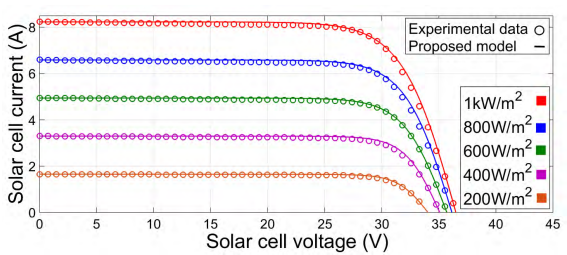
\includegraphics[width=\linewidth]{Imagenes/IEEE_V_Irr.png}
	\end{minipage}\hfill
	\begin{minipage}{0.5\textwidth}
		\centering
		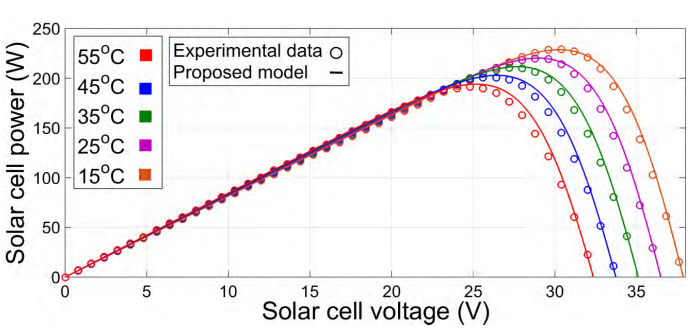
\includegraphics[width=\linewidth]{Imagenes/IEEE_T_Pwr.png}
	\end{minipage}
	\par\medskip
	
	\raggedright
	\footnotesize \textit{Nota.} Adaptado de \cite{Gonzalez2019Behavioral}.
	\label{fig:CurvasElectricasIrrTemp}
\end{figure}
    
\subsubsection{\textbf{Albedo:}} El albedo es la fracción de luz reflejada por el suelo, incide directamente en la cara posterior de los paneles bifaciales; un aumento en el índice de albedo eleva significativamente la corriente trasera, lo que genera una mayor ganancia bifacial y maximiza la producción total de energía del sistema \citep{Barreno2024}. En la Figura \ref{fig:CurvasElectricasAlbHum} (izquierda), se puede apreciar que, para todo el rango del coeficiente de albedo, la ganancia bifacial aumenta desde 5 a 25 \%.
    
\subsubsection{\textbf{Humedad y precipitaciones:}} Los altos niveles de humedad relativa aprovocan la refracción, reflexión y difracción de la luz solar. Esto atenúa la cantidad de radiación directa que logra alcanzar las celdas fotovoltaicas, reduciendo la corriente generada.   En contraste, aunque las precipitaciones reducen la irradiancia momentáneamente, actúan como el mecanismo de mitigación natural más efectivo, ya que lavan la superficie del panel, removiendo las partículas acumuladas causantes del \textit{soiling} \citep{Kazem2015Humidity}. En la Figura \ref{fig:CurvasElectricasAlbHum} (derecha), se observa que, para una diferencia de humedad del 30\% (entre 95 y 65 \%), el valor de la potencia aumenta de 50 a 105~W (+110\%),

\begin{figure}[H]
	
	\captionsetup{justification=raggedright, singlelinecheck=false, labelsep=none}
	
	\caption[Comportamiento eléctrico de un panel solar ante variaciones de albedo y humedad relativa.]{} 
	
	\textit{Comportamiento eléctrico de un panel solar ante variaciones de albedo (izquierda) y humedad relativa (derecha).} \par\medskip
	
	\begin{minipage}{0.5\textwidth}
		\centering
		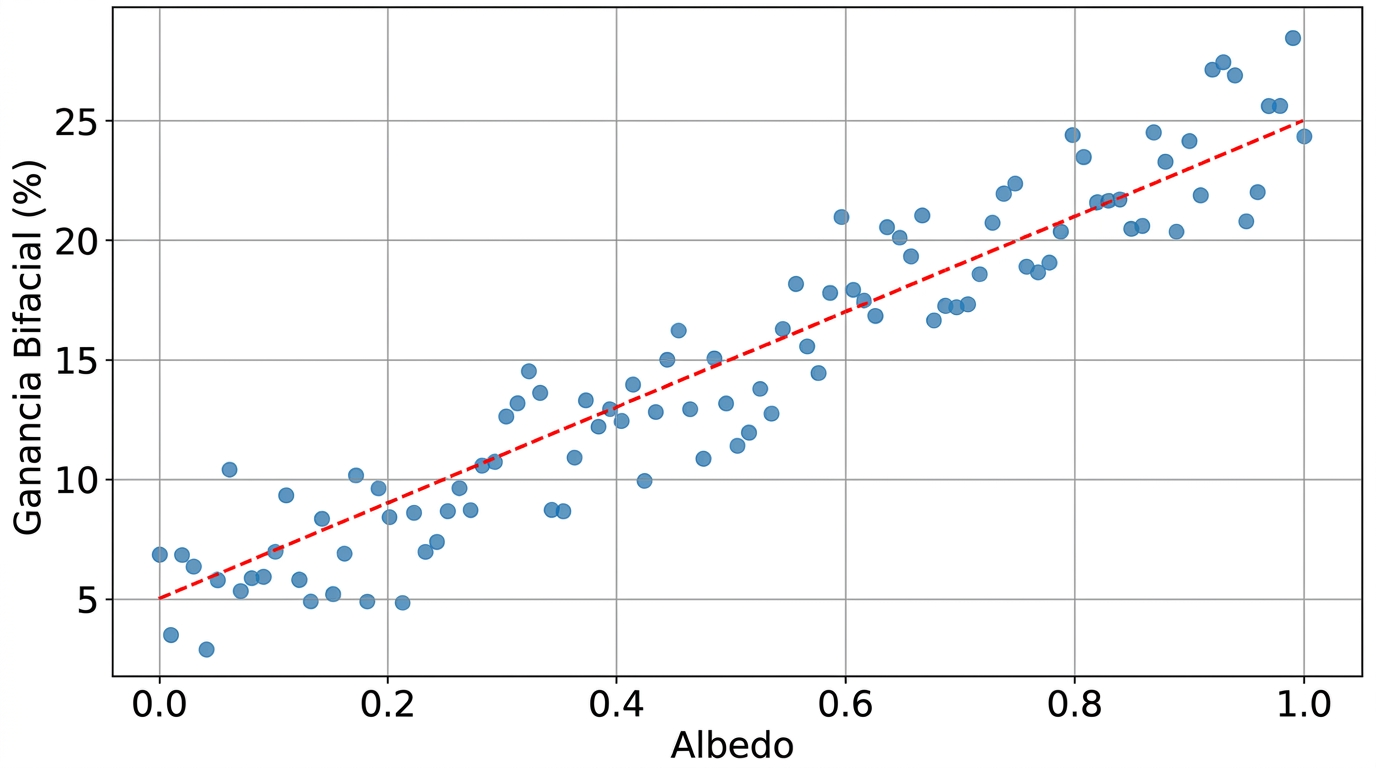
\includegraphics[width=\linewidth]{Imagenes/BARRENO_Alb_Ganancia.jpeg}
	\end{minipage}\hfill
	\begin{minipage}{0.5\textwidth}
		\centering
		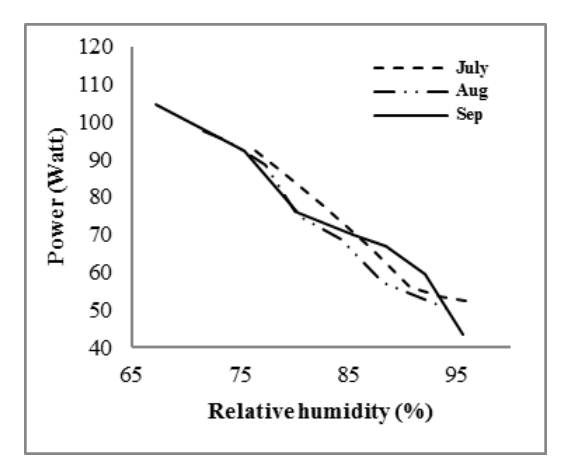
\includegraphics[width=\linewidth]{Imagenes/KAZEM_Hum_Pwr.png}
	\end{minipage}
	\par\medskip
	
	\raggedright
	\footnotesize \textit{Nota.} Adaptado de \cite{Barreno2024} (izquierda).Adaptado de \cite{Kazem2015Humidity} (derecha).
	\label{fig:CurvasElectricasAlbHum}
\end{figure}


\subsubsection{\textbf{Velocidad del viento:}} Presenta un efecto dual. Por un lado, cuando la velocidad del viento es moderada, este favorece el enfriamiento convectivo de los paneles, disipando el calor acumulado y reduciendo la temperatura de la celda, lo que incrementa la eficiencia y la potencia eléctrica de salida. 
Por otro lado, las ráfagas actúan como el principal transporte de partículas. Esto eleva las tasas de deposición de suciedad sobre los cristales, disminuyendo la generación de energía \citep{Vick_WindEffect}. En la Figura \ref{fig:Leow_Wind_Pwr} (derecha), se observa un una comparación cualitativa de la potencia de salida de dos paneles solares, con una diferencia promedio a lo largo de día de 7~W (11\% de potencia máxima de panel con aire).
    
\begin{figure}[H]
	\captionsetup{justification=raggedright, singlelinecheck=false, labelsep=none}
	\caption[Comparación entre la potencia generada a lo largo del día de paneles con y sin velocidad de viento.]{} 
	\textit{Comparación entre la potencia generada a lo largo del día de paneles con y sin velocidad de viento.} \par\medskip
	
	\centering
	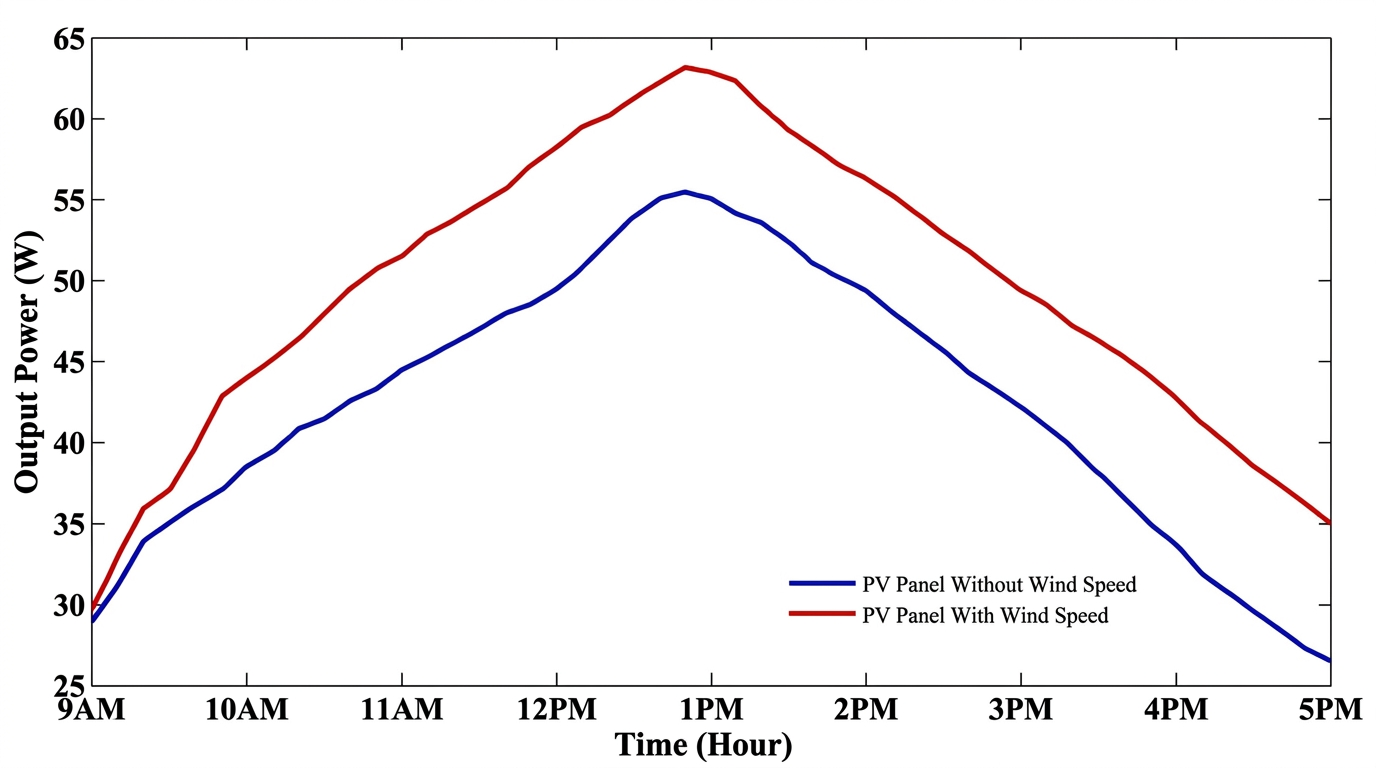
\includegraphics[width=0.8\textwidth]{Imagenes/Leow_Wind_Pwr.jpeg} \par\medskip
	\raggedright
	\footnotesize \textit{Nota.} Gráfico adaptado del artículo ``Influence of wind speed on the performance of photovoltaic
	panel'' \citep{Leow2019Wind}.
	\label{fig:Leow_Wind_Pwr}
\end{figure}

\subsubsection{\textbf{Pérdidas Técnicas:}} La eficiencia de esta conversión disminuye significativamente bajo condiciones operativas reales debido a dos fenómenos físicos principales. En primer lugar, el efecto térmico provoca que las celdas solares pierdan eficiencia a medida que su temperatura aumenta, ya que dicho incremento genera un coeficiente negativo en el voltaje de circuito abierto que reduce drásticamente la potencia máxima de salida \citep{Vieira2024}. 
Por otro lado, el fenómeno del soiling consiste en la acumulación de polvo, arena y contaminantes sobre la superficie de los módulos; esta capa de suciedad interfiere con la transmisión de la luz mediante procesos de absorción, reflexión y dispersión, generandopérdidas eléctricas que, al distribuirse de forma no uniforme, pueden derivar en la formación de puntos caliente” perjudiciales para la vida útil del panel y reducir severamente la rentabilidad de la instalación \citep{TesisJGB}.

\section{Marco referencial}

En esta sección se detallan las normativas, las condiciones topográficas y el entorno operativo bajo los cuales funcionará el robot autónomo de medición.

\subsection{Contexto normativo y estándares de medición}
Dado que el objetivo del vehículo es recolectar datos climáticos con validez industrial para el cálculo de índices de rendimiento, su instrumentación y métodos deben regirse estrictamente por la serie de estándares internacionales IEC 61724. Esta familia de normativas es la base para evaluar la capacidad y la energía de los sistemas fotovoltaicos. Dentro de esta serie, el principal referente para el diseño del hardware es la norma IEC 61724-1, la cual establece los requisitos para la monitorización del desempeño de sistemas fotovoltaicos y define las clases de exactitud exigidas para los sensores de irradiancia, temperatura y condiciones ambientales. Las exigencias de los parámetros más críticos definidos por esta norma, junto con su impacto en el proyecto, se detallan a continuación en la Tabla \ref{tab:requisitos_clase_ab}.

\begin{center}
\footnotesize
\begin{xltabular}{\textwidth}{|p{1.8cm}|>{\raggedright\arraybackslash}X|>{\raggedright\arraybackslash}X|p{2.8cm}|p{2.8cm}|}
\caption{Requisitos detallados por la Norma IEC 61724-1.}
\label{tab:requisitos_clase_ab} \\
\hline
\rowcolor[HTML]{D9E1F2} 
 &  &  & \multicolumn{2}{c|}{\textbf{Rango definido por la norma}} \\ \cline{4-5} 
\rowcolor[HTML]{D9E1F2} 
\multirow{-2}{*}{\textbf{Parámetro}} & \multirow{-2}{*}{\textbf{Descripción}} & \multirow{-2}{*}{\textbf{Impacto}} & \textbf{Clase A} & \textbf{Clase B} \\ \hline
\endfirsthead

\multicolumn{5}{c}%
{{\bfseries Continuación de la \tablename\ \thetable{}}} \\
\hline
\rowcolor[HTML]{D9E1F2} 
\textbf{Parámetro} & \textbf{Descripción} & \textbf{Impacto} & \textbf{Clase A} & \textbf{Clase B} \\ \hline
\endhead

\hline
\endfoot

\hline
\endlastfoot

\textbf{Clasificación} & Define las exigencias de exactitud y el diseño general para la recolección de datos. & Determina el rigor técnico y económico de la monitorización. & Alta exactitud (plantas grandes o a escala de red). & Exactitud media (instalaciones comerciales pequeñas o medianas). \\ \hline

\textbf{Intervalos} & Frecuencia de adquisición física (muestreo) y almacenamiento (registro). & Una alta frecuencia captura fluctuaciones rápidas y reduce la incertidumbre. & Muestreo máximo cada 5 segundos; Registro máximo cada 5 minutos, recomendado cada 1 minuto.. & Muestreo máximo cada 1 minuto; Registro máximo cada 5 minutos. \\ \hline

\textbf{Irradiancia} & Exigencias para los sensores de radiación incidente frontal y posterior. & Su exactitud define la incertidumbre final de la auditoría de rendimiento. & Piranómetro Clase A, espectralmente plano, incertidumbre menor al 2\%. & Piranómetro Clase C, incertidumbre menor al 3\%. \\ \hline

\textbf{Temperatura} & Medición térmica en la cara posterior del módulo y del aire circundante. & Dato vital para el cálculo de eficiencia corregido por temperatura. & \multicolumn{2}{p{5.6cm}|}{Resolución menor a $0,1^{\circ}\text{C}$ e incertidumbre entre $ \pm 1^{\circ}\text{C}$. El sensor de ambiente debe estar a 1 metro de distancia de fuentes térmicas.} \\ \hline

\textbf{Mitigación ambiental} & Protocolos de limpieza (\textit{soiling}) y sistemas contra rocío o escarcha. & Evita mediciones artificialmente bajas que afectarían el índice de rendimiento. & \multicolumn{2}{p{5.6cm}|}{Limpieza semanal o uso de tecnología automatizada de detección de \textit{soiling}} \\ \hline


\textbf{Salida de planta} & Medidor principal de potencia y energía neta inyectada a la red. & Determina el cumplimiento de garantías y la facturación real. & Medidores de Clase 0.2 S. & Medidores de Clase 0.5 S. \\ \hline

\end{xltabular}
\end{center}

\subsection{Condiciones topográficas y geográficas}
Las plantas solares a gran escala se pueden instalar en terrenos irregulares y montañosos que presentan una topografía compleja, lo cual propicia la generación de microclimas y fluctuaciones espaciales en la radiación incidente. El diseño de la base móvil y el sistema de locomoción del robot están directamente condicionados por las severas exigencias de este entorno natural; como los desniveles pronunciados, que pueden alcanzar hasta un 25\,\% \citep{Salinas2025}, como se puede observar en la Figura \ref{fig:PlantaPendiente} ; o los obstáculos geológicos, que incluye maleza, arena suelta, rocas, zanjas profundas causas por erosión y charcos de lodo \citep{Figgis2025}. Estas complejas condiciones justifican la adopción de sistemas de tracción con alta adaptabilidad y agarre, como los sistemas de orugas, necesarios para superar áreas inestables.

\begin{figure}[H]
	% Fuerza la alineación izquierda y quita los ":" después del número
	\captionsetup{justification=raggedright, singlelinecheck=false, labelsep=none}
	
	\caption[Imagen aérea de varias colinas cubiertas con paneles fotovoltaicos en Jinhua, provincia de Zhejiang, China.]{} 
	
	\textit{Imagen aérea de varias colinas cubiertas con paneles fotovoltaicos en Jinhua, provincia de Zhejiang, China.} \par\medskip
	
	\centering
	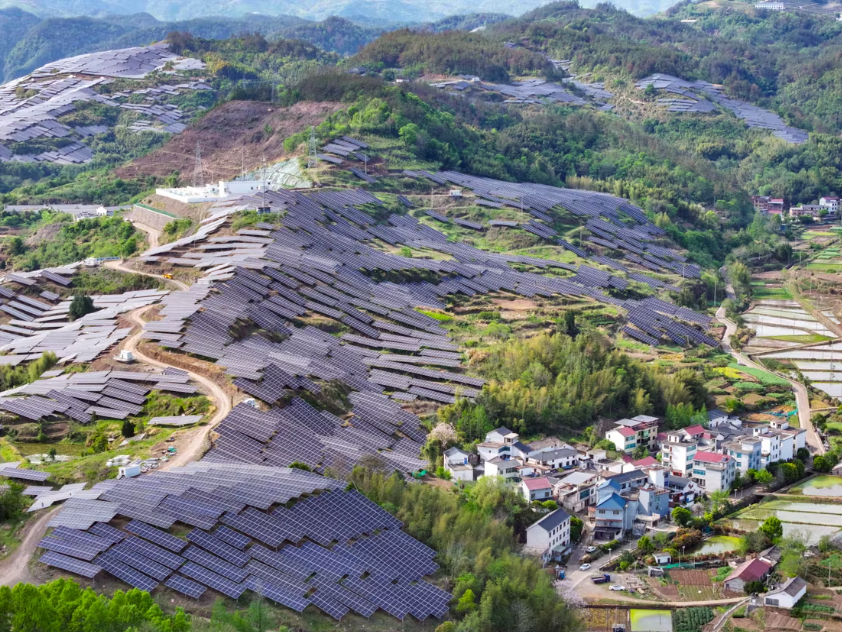
\includegraphics[width=0.6\textwidth]{Imagenes/PlantaPendiente.png} \par\medskip
	
	\raggedright
	\footnotesize \textit{Nota.} Fotografía adaptada sobre la noticia ``China, the energy transition superpower''  \citep{Pouille2025China}.
	\label{fig:PlantaPendiente}
\end{figure}

\subsection{Entorno operativo y tecnológico}
El contexto operativo y tecnológico define las estrechas interacciones del vehículo autónomo con la infraestructura civil y electromecánica propia de la planta. El trazado de las instalaciones modernas se apoya mayoritariamente en estructuras con seguidores solares de un solo eje, orientados de norte a sur y separados por pasillos que oscilan entre los 5 y 9 
de distancia \citep{ProyectoEjecutivo2024}.

En este escenario, la navegación autónoma del robot se verá restringida por obstáculos artificiales críticos. Entre ellos, la reducción del espacio transitable por la instalación de bandejas de distribución de cables y mallas reflectantes en el suelo, y la presencia de barras mecánicas entre las filas de los seguidores solares que impiden el libre tránsito transversal entre pasillos \citep{Figgis2025}. Todo ello exige que el robot disponga de un sistema de evitación de obstáculos robusto y una extrema precisión en su desplazamiento.

\section{Estado del arte} %PONER IMÁGENES EN LA TABLA

\subsection{Soluciones integrales}
En esta sección se analizan los sistemas mecatrónicos completos que intentan resolver el problema general de la inspección y medición dentro de los parques solares fotovoltaicos, sirviendo como referentes de diseño global para el vehículo terrestre autónomo propuesto.

\subsubsection{\textbf{Estación meteorológica fotovoltaica móvil (CN 216956405 U):}} Esta patente describe, como se ilustra en la Figura \ref{fig:CN216956405U} (izquierda), una estación climática (2) montada sobre una base con ruedas, vista en Figura la \ref{fig:CN216956405U} (derecha), que incluye soportes roscados, compuestos por una funda roscada y una varilla roscada, y placas o almohadillas estabilizadoras (5) que se despliegan hacia abajo para anclar el equipo en superficies desniveladas. El sistema destaca por su enfoque en la estabilización mecánica del equipo de medición, utilizando estos mecanismos de anclaje desplegables que aseguran que los sensores meteorológicos mantengan un plano de referencia adecuado al evitar que la base se incline, así como evita volcaduras el recorrido en terrenos con pendiente.
	
	\begin{figure}[H]
		
		\captionsetup{justification=raggedright, singlelinecheck=false, labelsep=none}
		
		\caption[Ilustraciones de estación meteorológica fotovoltaica móvil.]{} 
		
		\textit{Ilustraciones de estación meteorológica fotovoltaica móvil.} \par\medskip
		
		\begin{minipage}{0.4\textwidth}
			\centering
			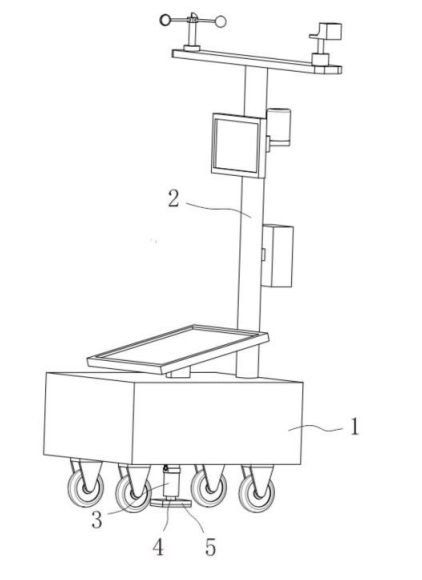
\includegraphics[width=\linewidth]{Imagenes/CN216956405U-1.png}
		\end{minipage}\hfill
		\begin{minipage}{0.4\textwidth}
			\centering
			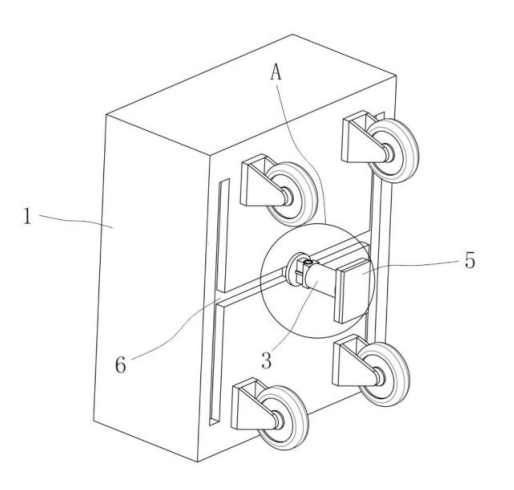
\includegraphics[width=\linewidth]{Imagenes/CN216956405U-2.png}
		\end{minipage}
		\par\medskip
		
		\raggedright
		\footnotesize \textit{Nota.} Adaptado de \cite{CN216956405U}.
		\label{fig:CN216956405U}
	\end{figure}
	
	
\subsubsection{\textbf{Vehículo de inspección para plantas de energía fotovoltaicas (CN 218409341 U):}} Es un vehículo terrestre no tripulado, mostrado en la Figura \ref{fig:CN218409341U}, montado sobre una base (1), equipado con ruedas de movimiento (21), paneles solares abatibles (12) para carga y un robusto mecanismo de amortiguación mediante resortes (20) en cajas para evitar daños en la instrumentación durante el tránsito. Esta patente representa una solución integral para la problemática, implementando el uso de paneles solares integrados para la recarga autónoma y sistemas de amortiguación para la protección de la instrumentación, lo que aseguraa la precisión de las mediciones dinámicas y prolonga la autonomía.
	
	\begin{figure}[H]
		\captionsetup{justification=raggedright, singlelinecheck=false, labelsep=none}
		
		\caption[Ilustración de vehículo de inspección con paneles solares y sistema de amortiguación.]{} 
		
		\textit{Ilustración de vehículo de inspección terrestre con paneles solares abatibles y mecanismo de amortiguación.} \par\medskip
		
		\centering
		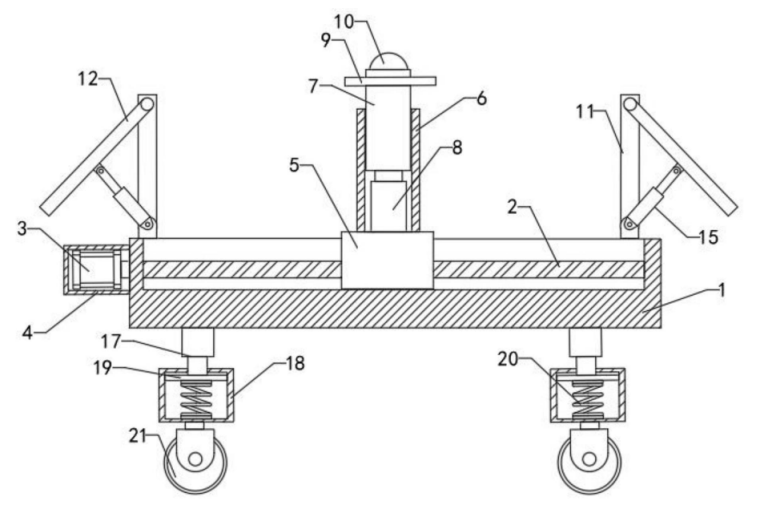
\includegraphics[width=0.75\textwidth]{Imagenes/CN218409341U.png} \par\medskip
		
		\raggedright
		\footnotesize \textit{Nota.} Adaptado de \cite{CN218409341U}.
		\label{fig:CN218409341U}
	\end{figure}
\subsubsection{\textbf{Vehículo de inspección para plantas fotovoltaicas en desiertos (CN 221163061 U):}} 
Este robot, como se ilustra en la Figura \ref{fig:CN221163061U}, cuenta con tracción de orugas (2) diseñada con ángulos de inclinación anti-deslizamiento (22) y está equipado con radar y sensores de viento, humedad y radiación o luz. La propuesta se alinea con el propósito general del proyecto, ya que el diseño integrado de un tren de tracción para terrenos desérticos acoplado a un sistema completo de sensores climáticos sirve como el principal punto de referencia comercial y tecnológico para validar la arquitectura y el alcance funcional del UGV de irradiancia propuesto.
	
	\begin{figure}[H]
		\captionsetup{justification=raggedright, singlelinecheck=false, labelsep=none}
		
		\caption[Ilustración de robot de inspección para estaciones fotovoltaicas en el desierto.]{} 
		
		\textit{Ilustración de robot de inspección con tracción de orugas y sensores climáticos para entornos desérticos.} \par\medskip
		
		\centering
		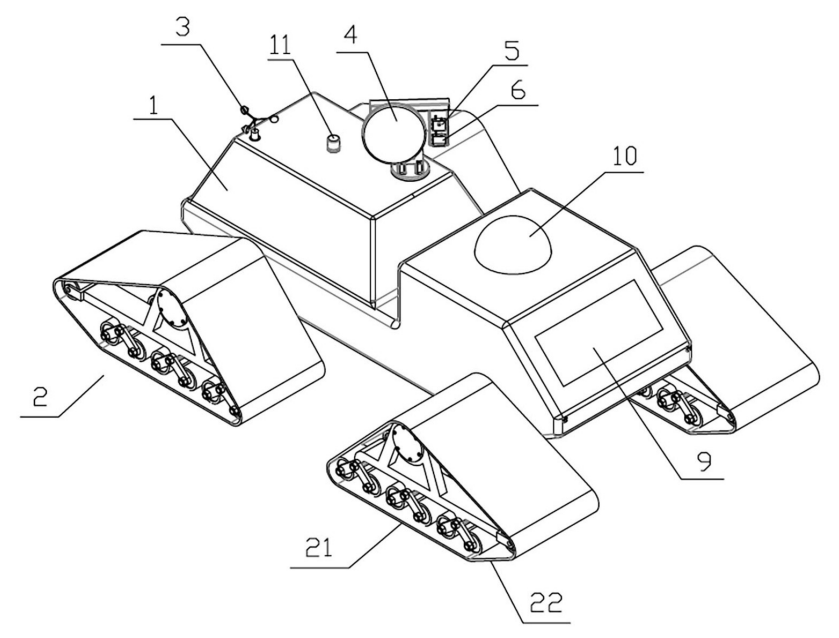
\includegraphics[width=0.7\textwidth]{Imagenes/CN221163061U.png} \par\medskip
		
		\raggedright
		\footnotesize \textit{Nota.} Adaptado de \citep{CN221163061U}.
		\label{fig:CN221163061U}
	\end{figure}
%%
%%
\begin{center}
\footnotesize
\begin{xltabular}{\textwidth}{|p{2.5cm}|>{\raggedright\arraybackslash}X|>{\raggedright\arraybackslash}X|>{\raggedright\arraybackslash}X|}
\caption{Análisis comparativo de Soluciones Integrales.}
\label{tab:estado_arte_integrales} \\
\hline
\rowcolor[HTML]{D9E1F2} 
\textbf{Referente} & \textbf{Principio de Funcionamiento} & \textbf{Aporte al Proyecto} & \textbf{Limitaciones} \\ \hline
\endfirsthead

\multicolumn{4}{c}%
{{\bfseries Continuación de la \tablename\ \thetable{}}} \\
\hline
\rowcolor[HTML]{D9E1F2} 
\textbf{Referente} & \textbf{Principio de Funcionamiento} & \textbf{Aporte al Proyecto} & \textbf{Limitaciones} \\ \hline
\endhead

\hline
\endfoot

\hline
\endlastfoot

%%
%%
%%

Estación meteorológica fotovoltaica móvil (CN 216956405 U)  & Estación sobre ruedas que emplea soportes roscados y almohadillas estabilizadoras de despliegue mecánico. & Proporciona mecanismos de nivelación y estabilización para asegurar el plano horizontal durante la lectura estática de sensores. & Tracción por ruedas ineficiente en terrenos irregulares; la nivelación pausada ralentiza el proceso de inspección dinámica. \\ \hline

Vehículo de inspección para plantas de energía fotovoltaicas (CN 218409341 U)  & Vehículo terrestre (UGV) con paneles solares abatibles y un mecanismo robusto de amortiguación con resortes en cajas. & Extiende la autonomía energética del robot e incorpora suspensión vital para proteger instrumentos sensibles de las vibraciones. & Locomoción por ruedas; carece de actuadores o mecanismos para limpiar los instrumentos ante la acumulación de polvo. \\ \hline

Vehículo de inspección para plantas fotovoltaicas en desiertos (CN 221163061 U)  & Chasis hermético propulsado por orugas antideslizantes, equipado con radar y sensores de radiación, viento y humedad. & Modelo de arquitectura mecatrónica base para un UGV desértico, combinando alta movilidad con medición climatológica. & Instrumentación estática en el chasis; no cuenta con ejes para adaptar la elevación o inclinación de los sensores a los paneles. \\ \hline

\end{xltabular}
\end{center}

%%
%%
\vspace{-1.5cm}
%%
\subsection{Soluciones parciales}
En esta sección se describen los componentes y subsistemas especializados que abordan necesidades técnicas específicas, clasificados según su funcionalidad.

\subsubsection{Robots para plantas fotovoltaicas}
\begin{itemize}
	\item \textbf{Vehículo de inspección terrestre inteligente para plantas fotovoltaicas (CN 119665962 A):} Esta patente, ilustrada en la Figura \ref{fig:CN119665962A&CN120057153A} (izquierda), describe un vehículo terrestre no tripulado cuya base (10) que incorpora soportes (20) y una carcasa superior (40) que aloja un panel fotovoltaico (30). Este vehículo está diseñado para la generación de mapas espaciales y la planificación de rutas globales de forma autónoma. El sistema integra algoritmos de navegación y percepción que le permiten realizar la recolección de datos ambientales en movimiento y la evasión de obstáculos en el terreno de manera autónoma.
	
	\item \textbf{Robot de inspección de alta transitabilidad para plantas fotovoltaicas (CN 120057153 A):} Ilustrado en la Figura \ref{fig:CN119665962A&CN120057153A} (derecha), se trata de un vehículo con tracción mediante ruedas activas (31) (con opción de incluir configuraciones de oruga) conectadas a módulos flotantes (32) de amortiguación con resortes oscilantes (35). Este diseño está concebido para operar en entornos con topografía irregular, como suelo desértico o con pendientes pronunciadas. Su configuración mecánica también incluye un brazo base (4) desplegable desde un compartimento de almacenamiento (2) para labores de inspección, el cual garantiza la estabilidad y movilidad del robot frente a obstáculos comunes en las plantas solares a gran escala, permitiéndole navegar entre los paneles incluso cuando la distancia al suelo es reducida.
	
	
	\begin{figure}[H]
		
		\captionsetup{justification=raggedright, singlelinecheck=false, labelsep=none}
		
		\caption[Ilustraciones de vehículo de inspección terrestre inteligente y robot de inspección de alta transitabilidad.]{} 
		
		\textit{Ilustraciones de vehículo de inspección terrestre inteligente y robot de inspección de alta transitabilidad.} \par\medskip
		
		\begin{minipage}{0.6\textwidth}
			\centering
			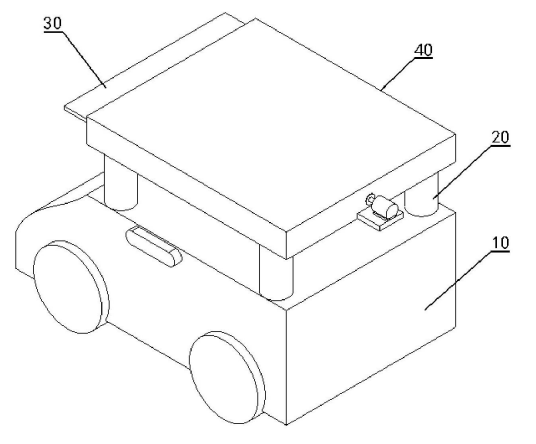
\includegraphics[width=\linewidth]{Imagenes/CN119665962A.png}
		\end{minipage}\hfill
		\begin{minipage}{0.5\textwidth}
			\centering
			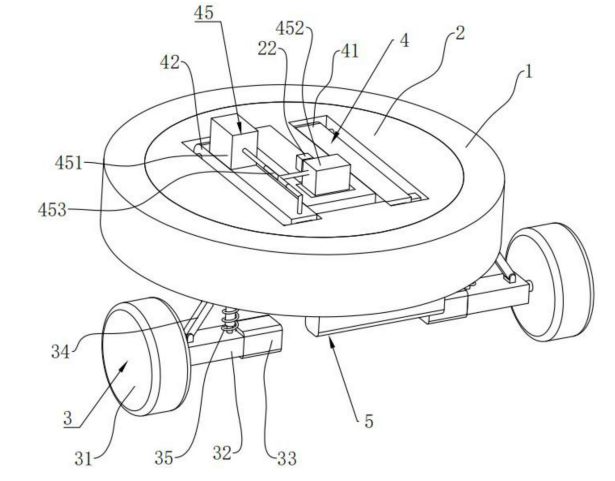
\includegraphics[width=\linewidth]{Imagenes/CN120057153A.png}
		\end{minipage}
		\par\medskip
		
		\raggedright
		\footnotesize \textit{Nota.} Adaptado de \cite{CN119665962A} (izquierda) y \cite{CN120057153A} (derecha).
		\label{fig:CN119665962A&CN120057153A}
	\end{figure}
	
	\item \textbf{Dispositivo de inspección automática para plantas fotovoltaicas (CN 220873036 U):} Este robot móvil, ilustrado en la Figura \ref{fig:CN220873036U}, comprende un cuerpo (1) sobre un mecanismo de desplazamiento, destaca por incorporar un motor (17) y un brazo giratorio o varilla (18) equipado con un cepillo o esponja (19) automatizado para la limpieza de los lentes de sus cámaras y mecanismos de captura de imágenes (8). Esta solución mecatrónica es esencial para mitigar el impacto del \textit{soiling} en los propios instrumentos del vehículo, como la plataforma de imágenes infrarrojas, asegurando la correcta lectura en las mediciones meteorológicas durante operaciones prolongadas en entornos con mucho polvo.
	
	\begin{figure}[H]
		\captionsetup{justification=raggedright, singlelinecheck=false, labelsep=none}
		
		\caption[Ilustración de vehículo de inspección con sistema de limpieza de sensores]{} 
		
		\textit{Ilustración de dispositivo de inspección automática con mecanismos de limpieza para sus instrumentos ópticos.} \par\medskip
		
		\centering
		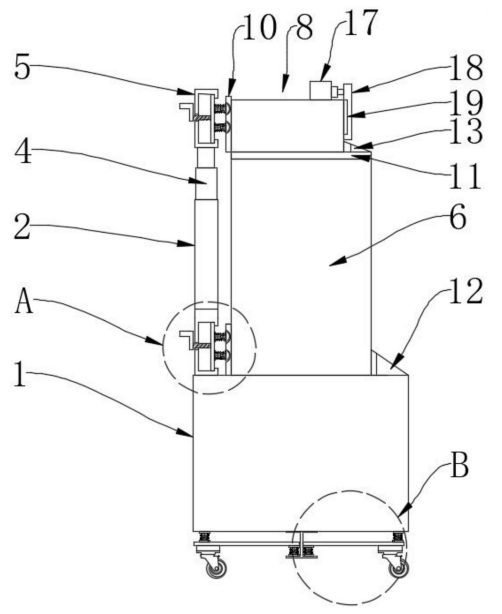
\includegraphics[width=0.4\textwidth]{Imagenes/CN220873036U.png} \par\medskip
		
		\raggedright
		\footnotesize \textit{Nota.} Adaptado de \cite{CN220873036U}.
		\label{fig:CN220873036U}
	\end{figure}
\end{itemize}

\begin{table}[H]
	\centering
	\footnotesize
	\caption{Análisis comparativo de Soluciones Parciales: Robots para plantas fotovoltaicas.}
	\label{tab:estado_arte_robots_pv}
	\begin{tabularx}{\textwidth}{|p{3.5cm}|>{\raggedright\arraybackslash}X|>{\raggedright\arraybackslash}X|>{\raggedright\arraybackslash}X|}
		\hline
		\rowcolor[HTML]{D9E1F2} 
		\textbf{Referente} & \textbf{Principio de Funcionamiento} & \textbf{Aporte al Proyecto} & \textbf{Limitaciones} \\ \hline
		Vehículo de inspección terrestre inteligente para plantas fotovoltaicas (CN 119665962 A) & Emplea algoritmos de control y datos ambientales para generar mapas espaciales y trazar rutas. & Aporta la arquitectura lógica para la navegación autónoma global y la evasión dinámica de obstáculos en la planta. & Cubre únicamente el dominio de software y control; no soluciona los retos mecánicos de tracción ni de captura física de datos. \\ \hline
		Robot de inspección de alta transitabilidad para plantas fotovoltaicas (CN 120057153 A) & Tren de locomoción basado en orugas acoplado a módulos flotantes de amortiguación para mantener el equilibrio. & Diseño mecánico ideal para sortear terrenos muy complejos, zanjas erosivas y pendientes de arena suelta. & Enfoque puramente cinemático y estructural; no integra sistemas de comunicación o instrumentación meteorológica. \\ \hline
		Dispositivo de inspección automática para plantas fotovoltaicas (CN 220873036 U) & Brazo robótico automatizado equipado con esponja o cepillo para frotar y limpiar los lentes de a bordo. & Estrategia de interacción física para mitigar de forma activa el soiling en los instrumentos durante largos recorridos. & Sistema optimizado para cámaras frontales; requiere rediseño para no dañar los domos de vidrio de los piranómetros. \\ \hline
	\end{tabularx}
\end{table}

\subsubsection{Robots para inspección de plantas de energía}
\begin{itemize}
	\item \textbf{Robot de inspección inteligente para plantas de energía (CN 215511023 U):} Esta plataforma móvil de orugas, como se ilustra en la Figura \ref{fig:CN215511023U&CN215701759U} (izquierda), integra un brazo mecánico (4) y un sistema de visión compuesto por una cámara óptica y un sensor infrarrojo. Una característica innovadora de este diseño es la inclusión de un sensor de nivel de líquidos (8) en su parte inferior, lo que permite al vehículo detectar y evadir charcos de lodo o zonas inundadas para proteger la integridad de sus componentes electrónicos, como el host de control central (7).
	
	\item \textbf{Robot de inspección para plantas de energía con mecanismo de corte (CN 215701759 U):} Este vehículo, como se ilustra en la Figura \ref{fig:CN215511023U&CN215701759U} (derecha) está equipado con un brazo giratorio (7) que posee un motor (8) y aspas de corte integradas (9). Este mecanismo permite al robot abrirse paso a través de vegetación o maleza que pueda obstruir las rutas de inspección, garantizando la continuidad del servicio de mantenimiento.
	
	
		\begin{figure}[H]
		
		\captionsetup{justification=raggedright, singlelinecheck=false, labelsep=none}
		
		\caption[Ilustraciones de robot de inspección con sensor de líquidos y robot de inspección con mecanismo de corte de maleza.]{} 
		
		\textit{Ilustraciones de robot de inspección con sensor de líquidos y robot de inspección con mecanismo de corte de maleza.} \par\medskip
		
		\begin{minipage}{0.5\textwidth}
			\centering
			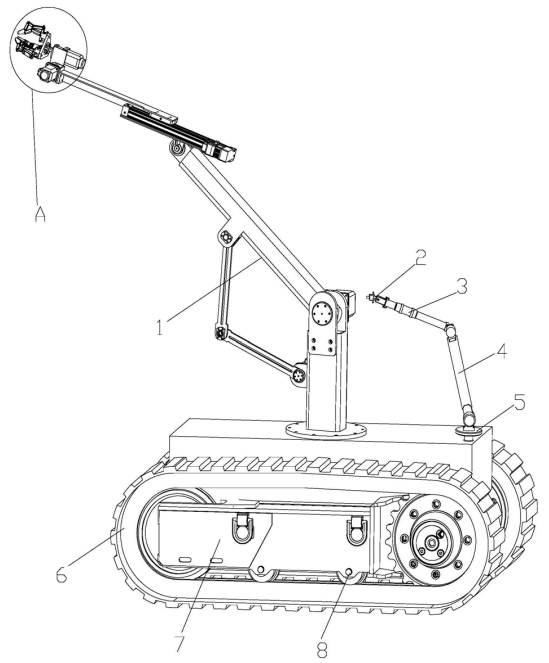
\includegraphics[width=\linewidth]{Imagenes/CN215511023U.png}
		\end{minipage}\hfill
		\begin{minipage}{0.6\textwidth}
			\centering
			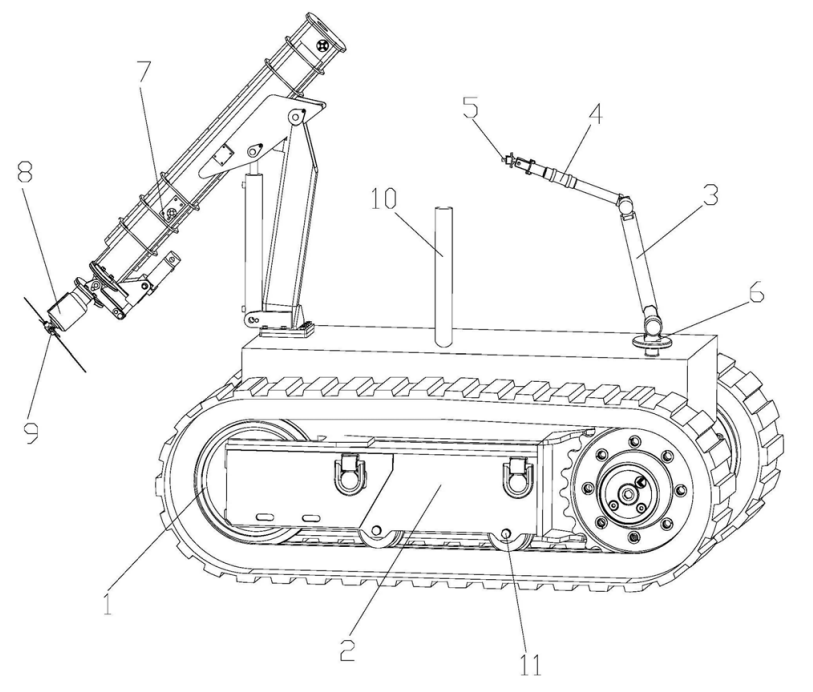
\includegraphics[width=\linewidth]{Imagenes/CN215701759U.png}
		\end{minipage}
		\par\medskip
		
		\raggedright
		\footnotesize \textit{Nota.} Adaptado de \cite{CN215511023U} (izquierda) y \cite{CN215701759U} (derecha).
		\label{fig:CN215511023U&CN215701759U}
	\end{figure}
	
	
	
\end{itemize}
%%%%%%

\begin{table}[H]
	\centering
	\footnotesize
	\caption{Análisis comparativo de Soluciones Parciales: Robots para inspección en general.}
	\label{tab:estado_arte_robots_general}
	\begin{tabularx}{\textwidth}{|p{3.5cm}|>{\raggedright\arraybackslash}X|>{\raggedright\arraybackslash}X|>{\raggedright\arraybackslash}X|}
		\hline
		\rowcolor[HTML]{D9E1F2} 
		\textbf{Referente} & \textbf{Principio de Funcionamiento} & \textbf{Aporte al Proyecto} & \textbf{Limitaciones} \\ \hline
		Robot de inspección inteligente para plantas de energía (CN 215511023 U) & Dispone de un sensor de nivel de líquidos en el tren inferior para detectar acumulación de agua. & Mecanismo de seguridad que funciona como alarma para evadir charcos de lodo, protegiendo la electrónica inferior. & Medida preventiva que detiene el avance; ante zonas altamente inundadas, el robot perdería su ruta planificada. \\ \hline
		Robot de inspección para plantas de energía con mecanismo de corte (CN 215701759 U) & Integra un brazo telescópico giratorio equipado con aspas de corte accionadas por motor eléctrico. & Brinda una solución mecánica para abrir paso en pasillos bloqueados por crecimiento de vegetación alta o maleza. & Alto consumo energético para la batería; aumenta la complejidad y el peso estructural frontal del vehículo. \\ \hline
	\end{tabularx}
\end{table}

\subsubsection{Estaciones meteorológicas para plantas fotovoltaicas}
\begin{itemize}
\item \textbf{Estación meteorológica solar multi-elemento (CN 216243088 U):} Esta estación meteorológica, como se ilustra en la Figura \ref{fig:CN216243088U&CN206638837U} (izquierda), emplea un trípode adaptativo (1) equipado con placas de refuerzo (3) y anclajes de fijación (14) con mecanismos de resorte. Este diseño, que soporta la caja meteorológica principal (11) y el panel solar (13), permite proporcionar una fijación mecánica rígida y estabilidad temporal a la estructura frente a ráfagas de viento fuertes, evitando que las vibraciones afecten la precisión de las mediciones ambientales.


\item \textbf{Sistema de monitoreo de estación meteorológica para módulos fotovoltaicos (CN 206638837 U):} El sistema, como se ilustra en la Figura \ref{fig:CN216243088U&CN206638837U} (derecha), propone una estructura con rieles y soportes móviles ,tales como la sección de colocación (1), que permiten ajustar la posición y el ángulo de los sensores y paneles solares (13). Esta funcionalidad facilita la alineación precisa de la instrumentación con el ángulo de las celdas solares fijas o dinámicas, permitiendo realizar mediciones exactas en el plano del panel fotovoltaico.




\begin{figure}[H]
	
	\captionsetup{justification=raggedright, singlelinecheck=false, labelsep=none}
	
	\caption[Ilustraciones de estación meteorológica con trípode adaptativo y estructura de soporte móvil con alineación.]{} 
	
	\textit{Ilustraciones de estación meteorológica con trípode adaptativo y estructura de soporte móvil con alineación.} \par\medskip
	
	\begin{minipage}{0.5\textwidth}
		\centering
		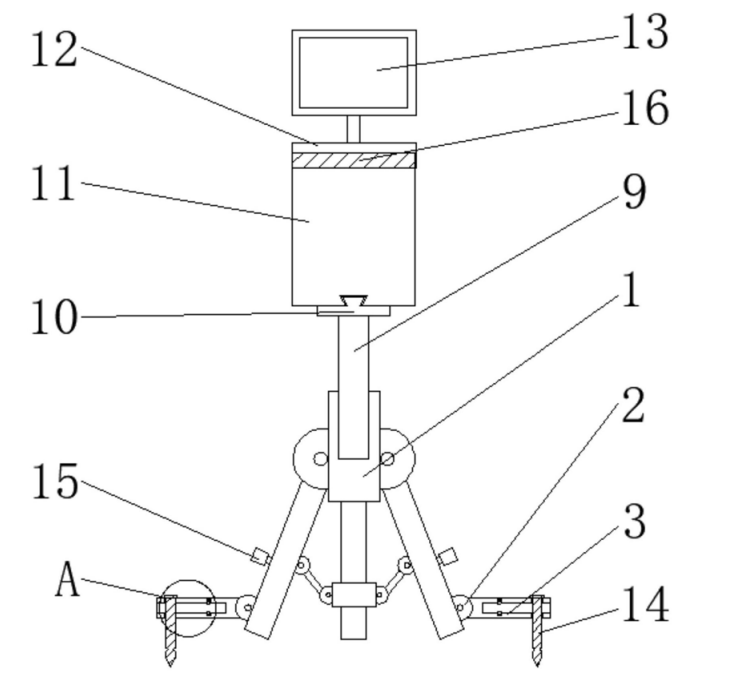
\includegraphics[width=\linewidth]{Imagenes/CN216243088U.png}
	\end{minipage}\hfill
	\begin{minipage}{0.5\textwidth}
		\centering
		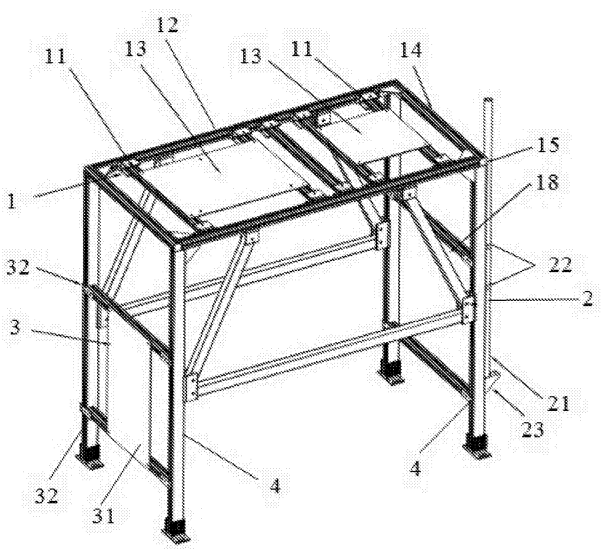
\includegraphics[width=\linewidth]{Imagenes/CN206638837U.png}
	\end{minipage}
	\par\medskip
	
	\raggedright
	\footnotesize \textit{Nota.} Adaptado de \cite{CN216243088U} (izquierda) y \cite{CN206638837U} (derecha).
	\label{fig:CN216243088U&CN206638837U}
\end{figure}

\item \textbf{Estación meteorológica simple para monitoreo ambiental (CN 206362955 U):} Se describe, como se ilustra en la Figura \ref{fig:CN206362955U&CN222047271U} (izquierda), un marco compacto (1) que integra sensores de radiación solar (7), instrumentos meteorológicos de cinco elementos para viento y otras variables (8), sensores de lluvia y sensores de temperatura, humedad y presión atmosférica mediante diversos mecanismos de fijación. Este modelo arquitectónico sirve como referencia para la distribución física del sistema de sensores a bordo de plataformas móviles, minimizando los efectos de sombreado mutuo entre instrumentos.


\item \textbf{Micro estación meteorológica automática y retractable (CN 222047271 U):} Esta patente describe, como se ilustra en la Figura \ref{fig:CN206362955U&CN222047271U} (derecha), una estación climática (2) montada sobre una base con ruedas (1) que incluye soportes roscado, compuestos por una funda roscada y una varilla roscada, y placas o almohadillas estabilizadoras (5) que se despliegan hacia abajo para anclar el equipo en superficies desniveladas. El sistema destaca por su enfoque en la estabilización mecánica del equipo de medición, utilizando estos mecanismos de anclaje desplegables que aseguran que los sensores meteorológicos mantengan un plano de referencia adecuado al evitar que la base se incline y eviten volcaduras durante la recolección de datos estáticos en terrenos con pendiente. 


\begin{figure}[H]
	
	\captionsetup{justification=raggedright, singlelinecheck=false, labelsep=none}
	
	\caption[Ilustraciones de estación meteorológica compacta y micro estación meteorológica automática con ajuste de altura.]{} 
	
	\textit{Ilustraciones de estación meteorológica compacta y micro estación meteorológica automática con ajuste de altura.} \par\medskip
	
	\begin{minipage}{0.6\textwidth}
		\centering
		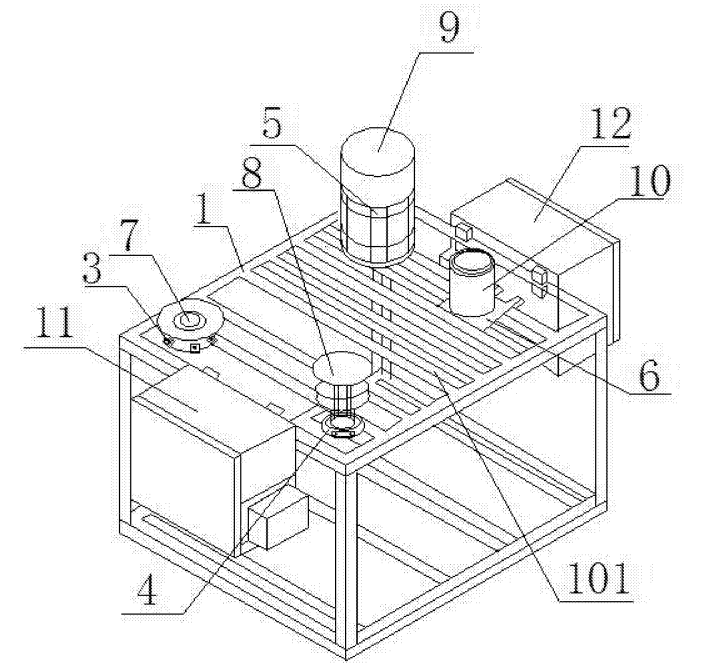
\includegraphics[width=\linewidth]{Imagenes/CN206362955U.png}
	\end{minipage}\hfill
	\begin{minipage}{0.2\textwidth}
		\centering
		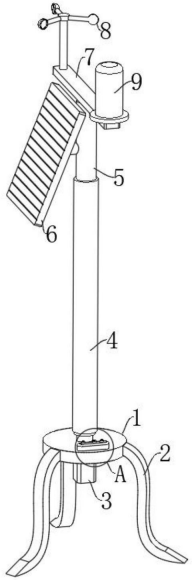
\includegraphics[width=\linewidth]{Imagenes/CN222047271U-1.png}
	\end{minipage}
	\par\medskip
	
	\raggedright
	\footnotesize \textit{Nota.} Adaptado de \cite{CN206362955U} (izquierda) y \cite{CN222047271U} (derecha).
	\label{fig:CN206362955U&CN222047271U}
\end{figure}

    \item \textbf{Instrumentación electrónica para una estación meteorológica automática (MX 2018007917 A):} Esta patente define la arquitectura de instrumentación basada en microcontroladores para el registro de variables como irradiancia global, temperatura, humedad y viento. El sistema establece la lógica de procesamiento y almacenamiento de datos en módulos locales, sirviendo de base para la programación de registro de datos embebidos.
    
    \item \textbf{MeteoPV:} Este producto comercial, visto en la Figura \ref{fig:MeteoPV} (izquierda), es una plataforma de monitorización del recurso solar diseñada específicamente para aplicaciones fotovoltaicas distribuidas. Funciona como un adquisidor de datos compacto con interfaz web integrada que facilita la configuración de piranómetros inteligentes, celdas de referencia y sensores de temperatura posterior, transmitiendo la información mediante protocolos industriales como Modbus RTU y TCP/IP hacia sistemas SCADA.
    
    	\begin{figure}[H]
    	\captionsetup{justification=raggedright, singlelinecheck=false, labelsep=none}
    	
    	\caption[Imagen de controlador MeteoPV.]{} 
    	
    	\textit{Imagen de controlador MeteoPV.} \par\medskip
    	
    	\centering
    	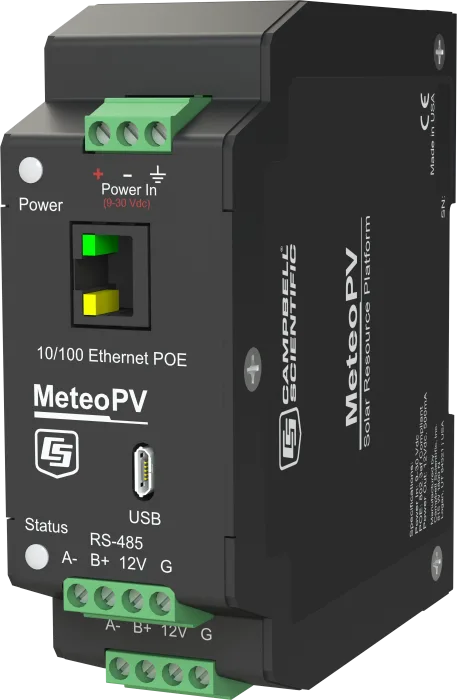
\includegraphics[width=0.3\textwidth]{Imagenes/MeteoPV.png} \par\medskip
    	
    	\raggedright
    	\footnotesize \textit{Nota.} Adaptado de \cite{MeteoPV}.
    	\label{fig:MeteoPV}
    \end{figure}
\end{itemize}

\begin{table}[H]
	\centering
	\footnotesize
	\caption{Análisis comparativo de Soluciones Parciales: Estaciones meteorológicas para plantas fotovoltaicas.}
	\label{tab:estado_arte_estaciones_pv}
	\begin{tabularx}{\textwidth}{|p{3.5cm}|>{\raggedright\arraybackslash}X|>{\raggedright\arraybackslash}X|>{\raggedright\arraybackslash}X|}
		\hline
		\rowcolor[HTML]{D9E1F2} 
		\textbf{Referente} & \textbf{Principio de Funcionamiento} & \textbf{Aporte al Proyecto} & \textbf{Limitaciones} \\ \hline
		Estación meteorológica solar multi-elemento (CN 216243088 U) & Trípode adaptativo con sistema de anclajes de bloqueo por resorte para afianzarse al suelo. & Alternativa de fijación temporal para dar rigidez al mástil de medición frente a ráfagas de viento fuertes. & Naturaleza estática; su despliegue mecánico requiere que el vehículo se detenga por completo para realizar lecturas. \\ \hline
		Sistema de monitoreo de estación meteorológica para módulos fotovoltaicos (CN 206638837 U) & Marco estructural equipado con rieles y soportes móviles que ajustan la orientación de los piranómetros. & Principio geométrico aplicable para alinear los sensores con el ángulo de inclinación de los seguidores solares. & Sistema de ajuste manual; para el UGV requerirá integración con actuadores motorizados para operación autónoma. \\ \hline
		Estación meteorológica simple para monitoreo ambiental (CN 206362955 U) & Estructura estática compacta que integra en un solo marco sensores de radiación, viento, lluvia y temperatura. & Referencia para la distribución física de la suite de sensores a bordo de plataformas móviles, minimizando sombreados. & Diseño estático fijo que no permite la adaptación dinámica al ángulo de incidencia solar. \\ \hline
		Instrumentación electrónica para una estación meteorológica automática (MX 2018007917 A) & Arquitectura basada en microcontroladores para el registro de variables climáticas en módulos locales SD. & Establece la lógica de procesamiento y almacenamiento de datos para registradores de datos embebidos. & Sistema básico de registro sin capacidades de telemetría de largo alcance integradas. \\ \hline
		Micro estación meteorológica automática y retractable (CN 222047271 U) & Mástil de medición basado en un tubo telescópico extendido verticalmente por un motor eléctrico. & Permite elevar instrumentos para evadir las turbulencias y el polvo generado por el chasis móvil. & Elevar el mástil modifica el centro de gravedad del robot, lo que podría desestabilizarlo al transitar sobre pendientes. \\ \hline
		Plataforma MeteoPV & Datalogger comercial que concentra datos de sensores inteligentes y los transmite mediante Modbus RTU/TCP. & Prototipo comercial directo para la arquitectura de adquisición del UGV; asegura inmunidad ante el ruido de los motores. & Es un módulo pasivo diseñado para montaje estandarizado; requiere gestión de disipación térmica y no controla locomoción. \\ \hline
	\end{tabularx}
\end{table}
\subsubsection{Ajuste de orientación para sensores de irradiancia}

\begin{itemize}
	
	
    \item \textbf{Seguidor solar SOLYS2} Este producto, visto en la Figura \ref{fig:ZippZonen_Tracker&Radiometer} (derecha) es un seguidor solar de alta precisión que incluye un receptor GPS integrado para la configuración automática de las coordenadas geográficas y la hora. Su diseño permite un seguimiento exacto para orientar instrumentos de medición directa, eliminando la necesidad de ajustes manuales constantes o sincronización por computadora externa.
	
    
    \item \textbf{Kit de montaje para piranómetro con inclinación ajustable} Este producto, visto en la Figura \ref{fig:ZippZonen_Tracker&Radiometer}, trata de un soporte mecánico con escala graduada diseñado para montar piranómetros en ángulos de inclinación específicos de $0^{\circ}$ a $90^{\circ}$. Este kit permite igualar manualmente la inclinación de los sensores con la de los paneles fotovoltaicos fijos, asegurando que la irradiancia medida sea la misma que incide sobre la superficie de generación.
    
    
    \begin{figure}[H]
    	
    	\captionsetup{justification=raggedright, singlelinecheck=false, labelsep=none}
    	
    	\caption[Kit de montaje para piranómetro con inclinación ajustable de KIPP \& ZONEN.]{} 
    	
    	\textit{Fotos de módulo controlador MeteoPV y seguidor solar SOLYS2 de KIPP \& ZONEN.} \par\medskip
    	
    	\begin{minipage}{0.5\textwidth}
    		\centering
    		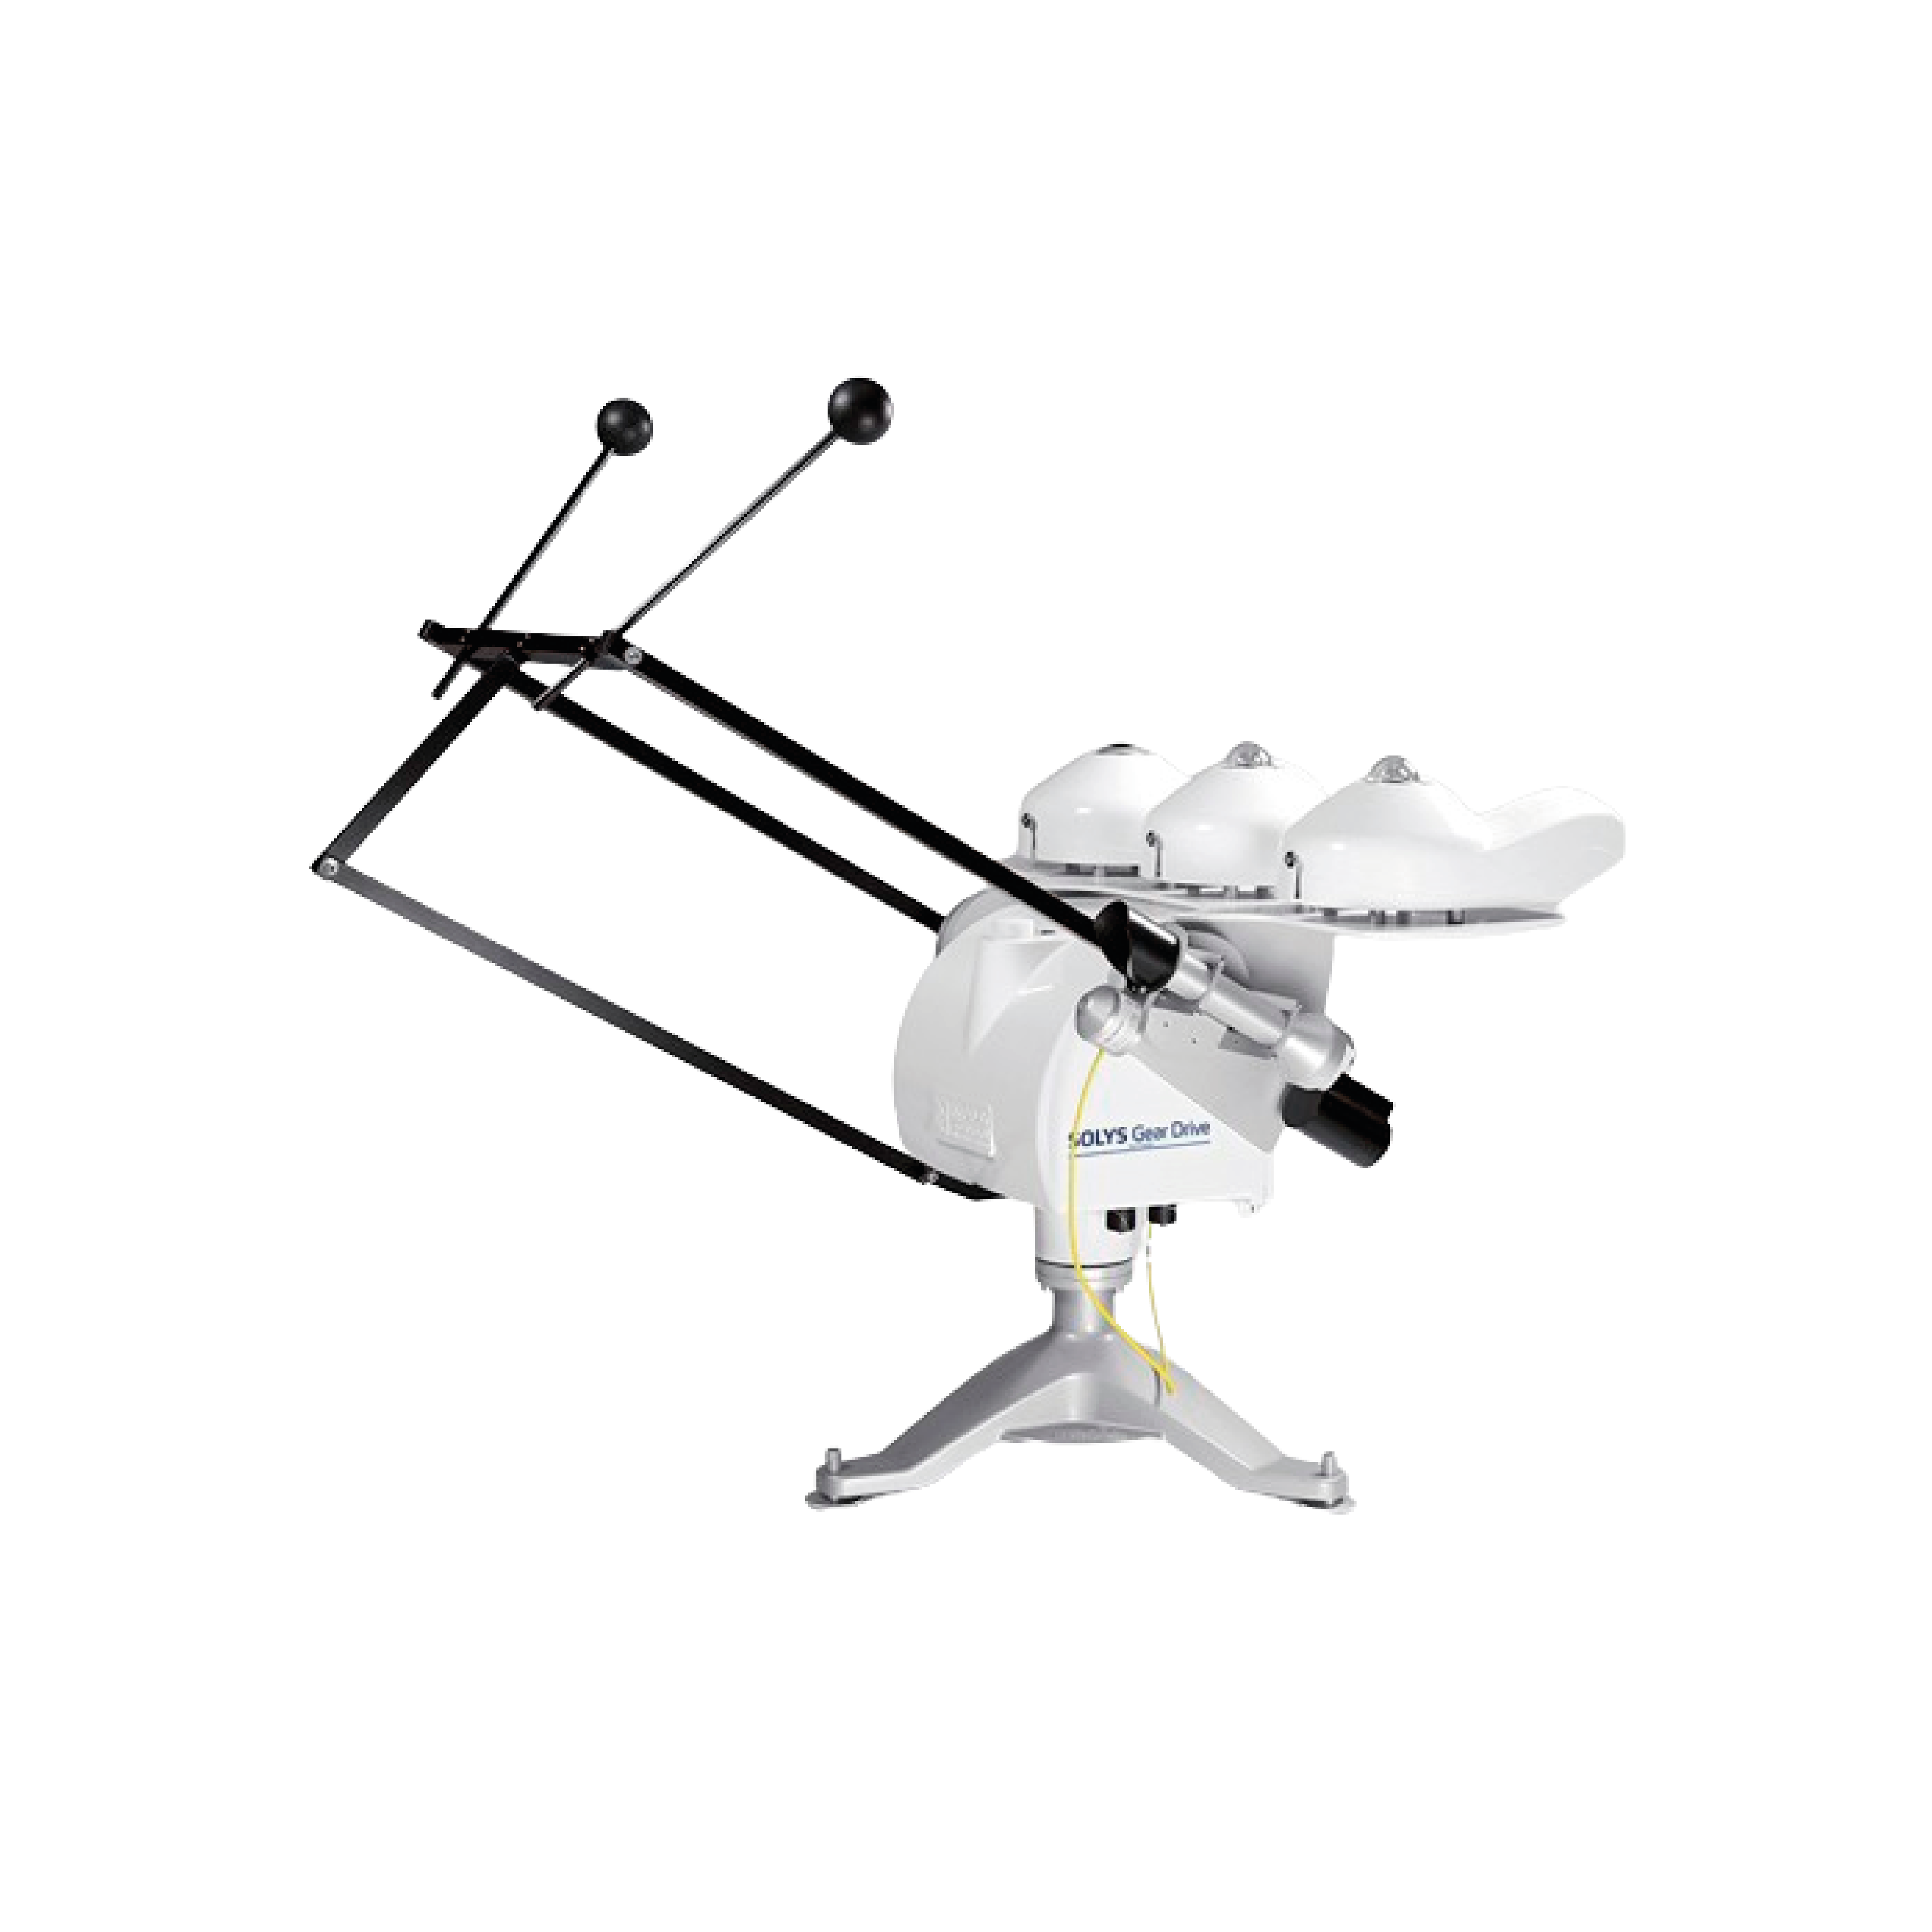
\includegraphics[width=\linewidth]{Imagenes/KippZonen_SunTrackers.png}
    	\end{minipage}\hfill
    	\begin{minipage}{0.5\textwidth}
    		\centering
    		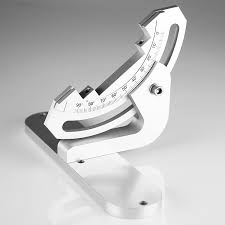
\includegraphics[width=\linewidth]{Imagenes/KippZonen_Radiometer.jpg}
    	\end{minipage}
    	\par\medskip
    	
    	\raggedright
    	\footnotesize \textit{Nota.} Adaptado de \cite{KippZonen_SunTrackers} (izquierda) y \cite{KippZonen_Radiometer} (derecha).
    	\label{fig:ZippZonen_Tracker&Radiometer}
    \end{figure}
    
    
\end{itemize}

\begin{table}[H]
	\centering
	\footnotesize
	\caption{Análisis comparativo de Soluciones Parciales: Sistemas de comunicación para datos meteorológicos.}
	\label{tab:estado_arte_comunicacion}
	\begin{tabularx}{\textwidth}{|p{3.5cm}|>{\raggedright\arraybackslash}X|>{\raggedright\arraybackslash}X|>{\raggedright\arraybackslash}X|}
		\hline
		\rowcolor[HTML]{D9E1F2} 
		\textbf{Referente} & \textbf{Principio de Funcionamiento} & \textbf{Aporte al Proyecto} & \textbf{Limitaciones} \\ \hline
		Estación meteorológica avanzada IoT (SK 302020 A3) & Sistema meteorológico IoT con un avanzado bloque de gestión y recuperación de baterías (BMS). & Permite administrar la energía de los sensores de forma independiente a otros sistemas motrices del vehículo. & No aborda aspectos de navegación o estabilidad mecánica requeridos para la movilidad en planta. \\ \hline
		Sistema de monitoreo de plantación basado en LoRa (CN 208458788 U) & Utiliza nodos sensores móviles y fijos conectados mediante red inalámbrica LoRa a un gateway central. & Permite la transmisión de datos a largas distancias con bajo consumo, ideal para supervisión remota en plantas extensas. & La latencia inherente a LoRa puede limitar la frecuencia de muestreo en inspecciones de alta velocidad. \\ \hline
		Método de posicionamiento para robots móviles (CN 116405876 A) & Emplea módulos LoRa para comunicación y cálculo de ubicación mediante intensidad de señal y tiempo de llegada. & Proporciona un método de localización en tiempo real para el seguimiento preciso de la ruta del vehículo. & Requiere la instalación de múltiples gateways distribuidos en el área operativa para garantizar precisión. \\ \hline
	\end{tabularx}
\end{table}


\subsubsection{Sistemas de comunicación para datos meteorológicos}
\begin{itemize}
    \item \textbf{Estación meteorológica avanzada IoT (SK 302020 A3):} Esta solución detalla un sistema meteorológico dividido en bloques funcionales, donde resalta un bloque avanzado de gestión y recuperación de baterías. Este esquema permite administrar la energía de los sensores de forma independiente a otros sistemas motrices, garantizando la continuidad de la toma de datos IoT incluso en condiciones de baja carga.
    
    \item \textbf{Sistema de monitoreo de plantación basado en LoRa (CN 208458788 U):} Este sistema utiliza la tecnología de comunicación inalámbrica LoRa para conectar múltiples nodos sensores, tanto móviles como fijos, con un gateway central. La arquitectura permite transmitir datos ambientales de irradiancia, viento y temperatura a largas distancias con bajo consumo energético, facilitando la supervisión remota a través de plataformas en la nube.
    
    \item \textbf{Método de posicionamiento para robots móviles (CN 116405876 A):} El método emplea módulos LoRa instalados en robots móviles que se comunican con gateways fijos distribuidos en el área de operación. Mediante el análisis de la intensidad de señal y el tiempo de llegada, el sistema permite determinar la ubicación precisa del vehículo en tiempo real y transmitir sus datos operativos hacia un servidor de control.
\end{itemize}

%

\begin{table}[H]
	\centering
	\footnotesize
	\caption{Análisis comparativo de Soluciones Parciales: Ajuste de orientación para sensores de irradiancia.}
	\label{tab:estado_arte_ajuste_sensores}
	\begin{tabularx}{\textwidth}{|p{3.5cm}|>{\raggedright\arraybackslash}X|>{\raggedright\arraybackslash}X|>{\raggedright\arraybackslash}X|}
		\hline
		\rowcolor[HTML]{D9E1F2} 
		\textbf{Referente} & \textbf{Principio de Funcionamiento} & \textbf{Aporte al Proyecto} & \textbf{Limitaciones} \\ \hline
		Seguidor solar SOLYS2 & Seguidor solar automático con receptor GPS integrado para configuración autónoma de ubicación y tiempo. & Referencia para el seguimiento exacto de la trayectoria solar para instrumentos de medición directa. & Elevado peso y costo para ser integrado en una plataforma móvil de exploración dinámica. \\ \hline
		Kit de montaje para piranómetro con inclinación ajustable & Soporte mecánico con escala graduada para montaje de piranómetros en ángulos de $0^{\circ}$ a $90^{\circ}$. & Permite igualar manualmente la inclinación de los sensores con la de los paneles fotovoltaicos fijos (Plano POA). & Requiere intervención humana para el ajuste del ángulo de inclinación inicial. \\ \hline
	\end{tabularx}
\end{table}
%
%
\section{Identificación de usuarios}

El diseño y la implementación del robot autónomo para la medición de variables climáticas involucra a diversos actores dentro del ecosistema de una planta solar fotovoltaica a gran escala. Identificar a estos usuarios y comprender sus necesidades específicas es fundamental para establecer los requerimientos de diseño del sistema mecatrónico. Los agentes involucrados se clasifican en usuarios directos e indirectos.

Para estructurar visualmente el nivel de interacción de cada actor con el equipo y sus datos, se emplea un Stakeholder Map basado en un modelo concéntrico (ver \ref{fig:StakeholderMap}). Esta herramienta clasifica a los agentes en tres niveles de proximidad: el núcleo operativo, el entorno comercial y de gestión y la periferia normativa e institucional.

    	\begin{figure}[H]
	\captionsetup{justification=raggedright, singlelinecheck=false, labelsep=none}
	
	\caption[Stakeholder Map con usuario principal, usuarios directos e indirectos]{} 
	
	\textit{Stakeholder Map con usuario principal, usuarios directos e indirectos} \par\medskip
	
	\centering
	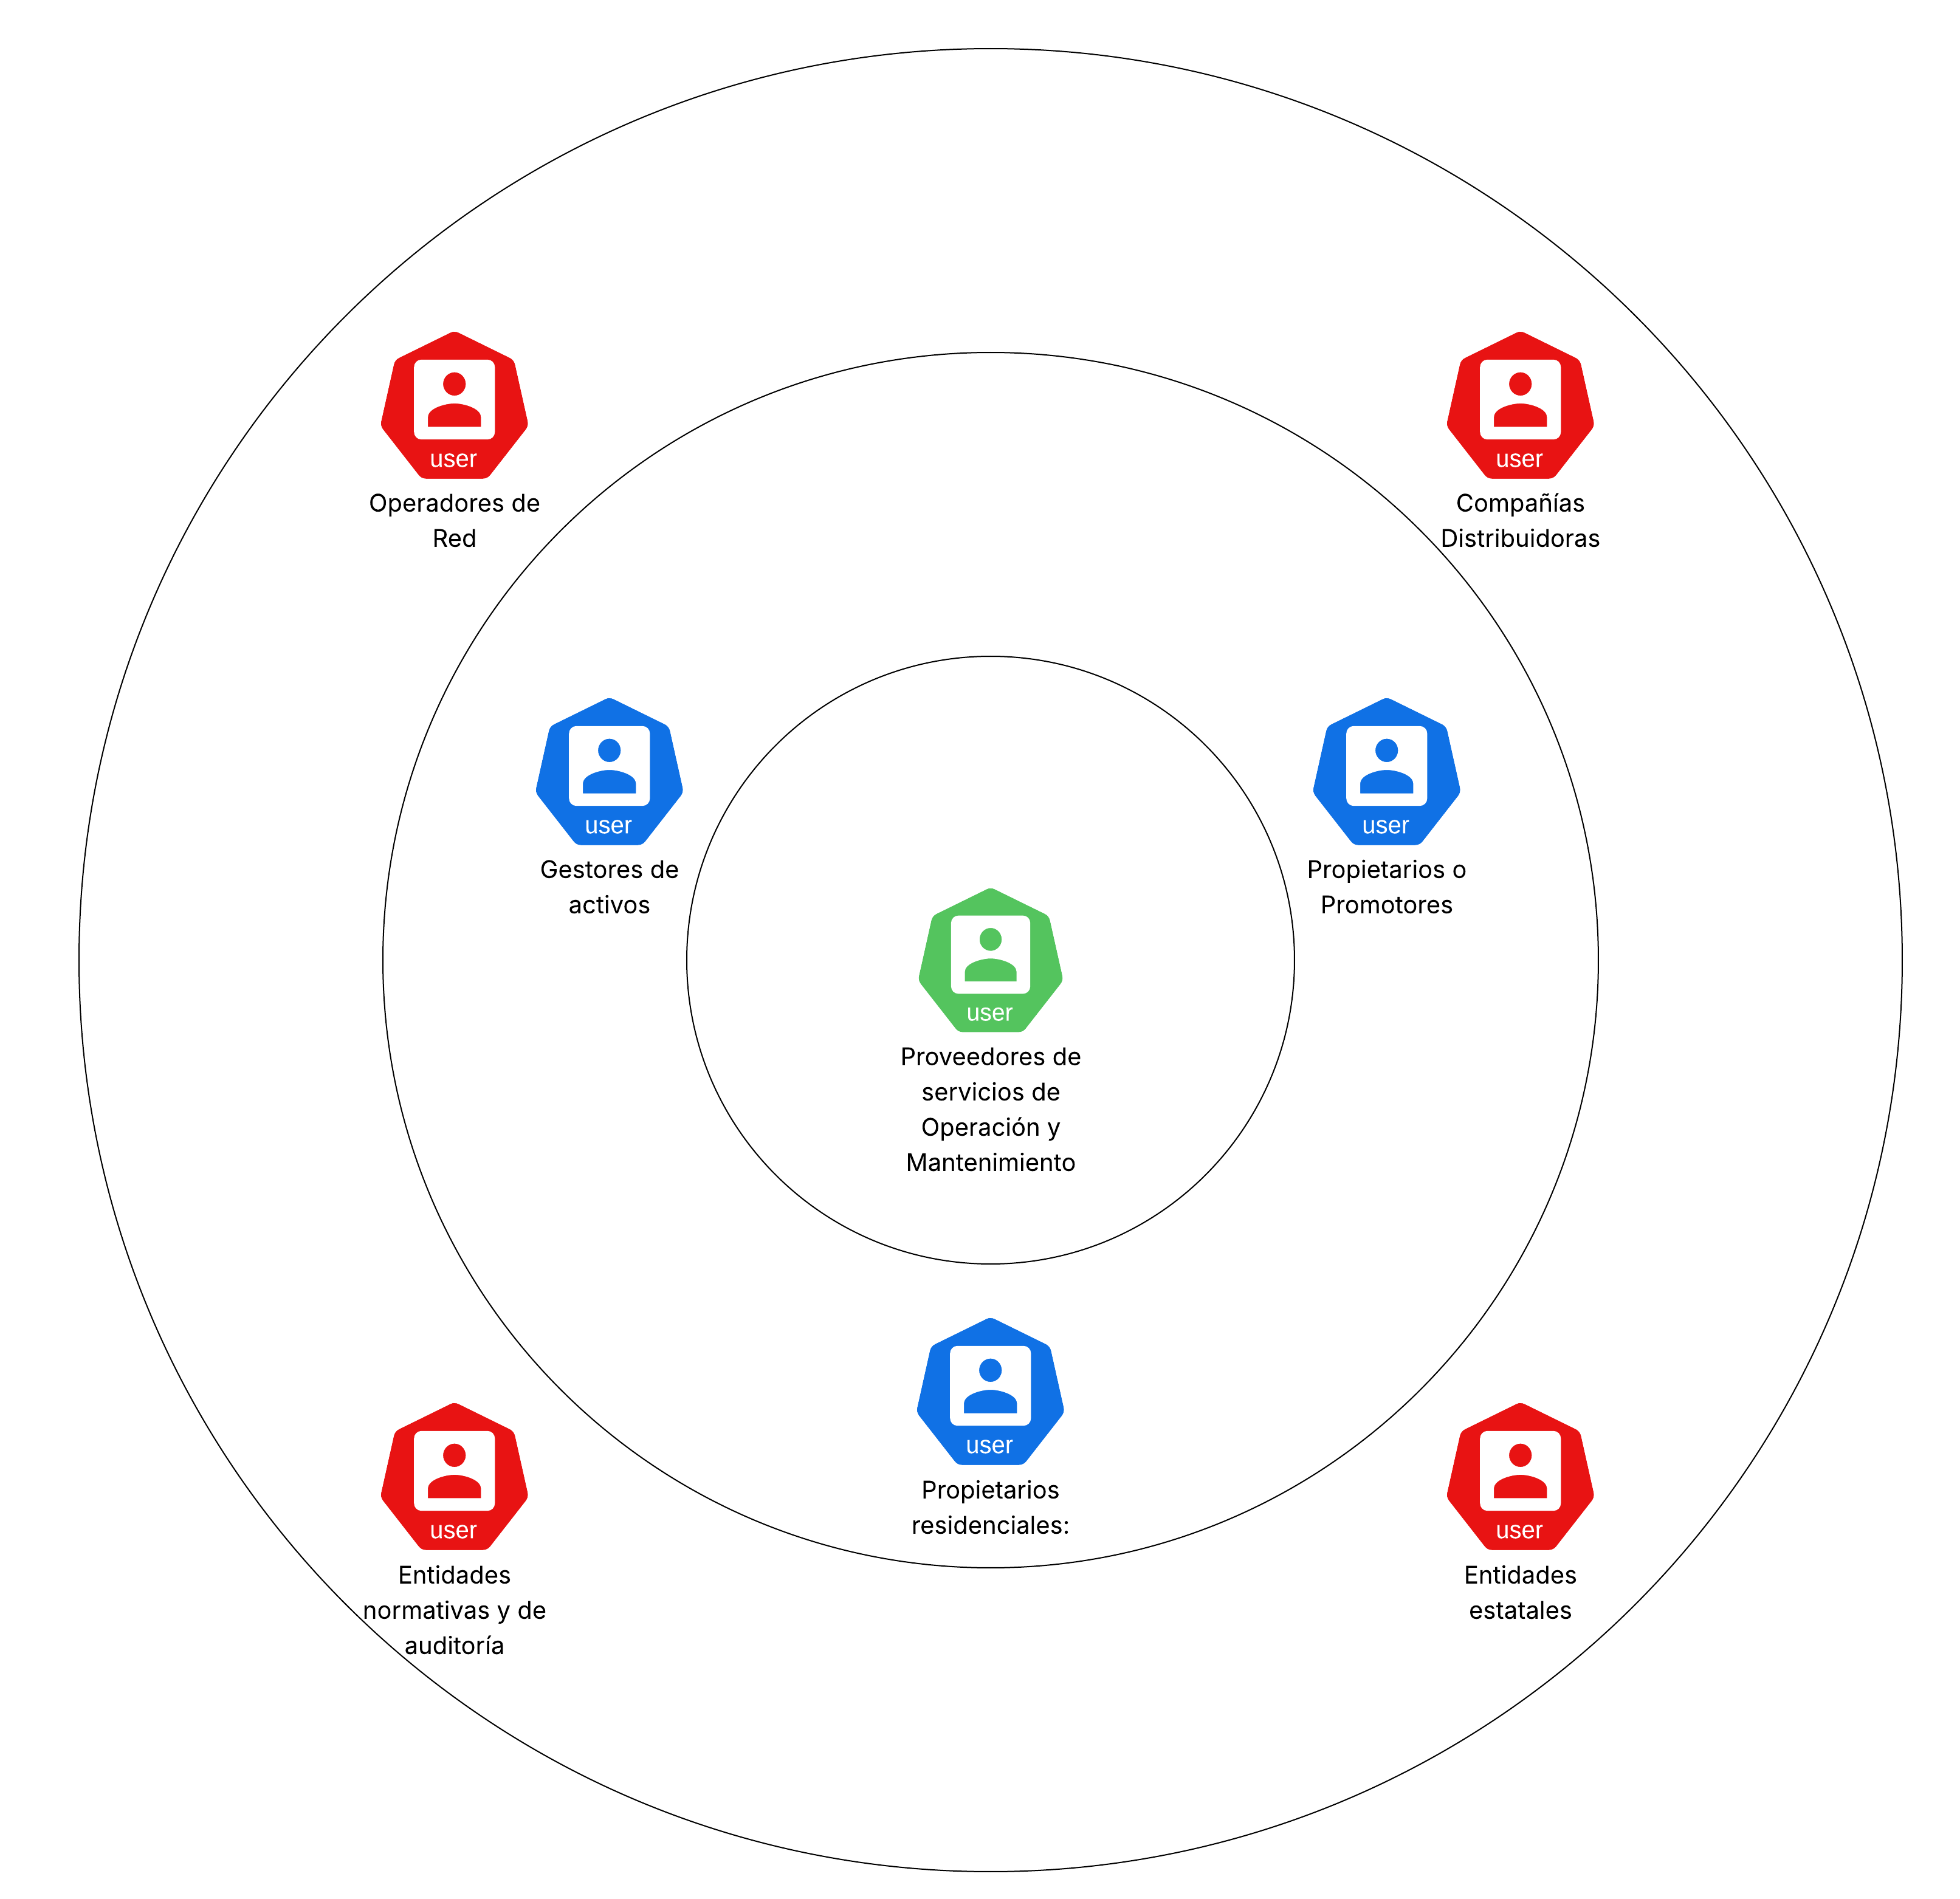
\includegraphics[width=\textwidth]{Imagenes/StakeholderMap.png} \par\medskip
	
	\raggedright
	\footnotesize \textit{Nota.} Elaboración propia.
	\label{fig:StakeholderMap}
\end{figure}

\subsection{Usuario principal}

El usuario principal es aquel cuyas necesidades sirven como base principal de los requerimientos del proyecto.
\begin{itemize}
	
	
 \item \textbf{Proveedores de servicios de Operación y Mantenimiento (O\&M):} Personal técnico y de ingeniería encargado del funcionamiento diario de la planta. Su necesidad principal es transicionar de un enfoque de mantenimiento correctivo a uno predictivo y preventivo. Además, necesitan capturar datos climáticos precisos para cuantificar objetivamente las pérdidas por ensuciamiento y optimizar así sus ciclos de limpieza \citep{TesisJGB}.
\end{itemize}

\subsection{Usuarios directos}
Estos usuarios interactúan directamente con los datos generados por el sistema o dependen de ellos para la gestión técnica y comercial de la planta:

\begin{itemize}

    
    \item \textbf{Gestores de activos}: Profesionales o entidades responsables de la gestión comercial y financiera de la inversión en energía renovable, así como de la supervisión y control de las actividades técnicas delegadas a los contratistas de O\&M. Para llevar a cabo su labor de auditoría, requieren que la recolección de datos capture la variabilidad climática adecuada en el terreno. Esto les permite evaluar la salud de los activos, calcular con exactitud los indicadores clave de rendimiento, y comparar de forma objetiva si el rendimiento energético medido en el parque cumple con las expectativas de diseño \citep{ProyectoEjecutivo2024}.
    
    \item \textbf{Propietarios o Promotores}: Entidades inversoras o corporaciones dueñas de la instalación fotovoltaica que financian y promueven el proyecto desde su concepción. Su necesidad principal es salvaguardar la viabilidad del proyecto a largo plazo, reducir costos y prolongar la vida útil de los equipos para maximizar la rentabilidad de la infraestructura. Para ellos, disponer de mediciones climáticas dinámicas y representativas se traduce en una reducción de la incertidumbre operativa y financiera, garantizando que el retorno de inversión esté respaldado por datos confiables sobre el recurso solar\citep{ProyectoEjecutivo2024}.
    
    \item \textbf{Propietarios residenciales (Personas naturales)}: : Representan a los individuos que poseen plantas fotovoltaicas personales, ya sean sistemas de generación distribuida orientados al autoconsumo o sistemas \textit{off-grid}. Aunque estas instalaciones operan a una escala mucho menor enfocada en la microgeneración, estos usuarios comparten la necesidad de contar con sistemas de medición accesibles que les permitan contrastar las variables climáticas locales con la producción de sus módulos. 
\end{itemize}

\subsection{Agentes indirectos}
Estos actores imponen las condiciones y los estándares de calidad bajo los cuales los datos del robot deben ser recolectados y transmitidos:

\begin{itemize}

    \item \textbf{Operadores de Red:} Entidades encargadas de la gestión de la red eléctrica nacional o regional. Necesitan que la planta fotovoltaica garantice una inyección de potencia predecible. La recolección dinámica de datos climáticos ayuda a prever fluctuaciones en la generación, permitiendo que los sistemas de control regulen adecuadamente la potencia activa y reactiva en el punto de interconexión (Kenemora Solar, 2024).
    
    \item \textbf{Compañías Distribuidoras:} Entidades encargadas de la facturación, los contratos y atención al cliente tanto a pequeña como mediana escala. Su principal interés es conocer al detalle el costo de la energía eléctrica para poder generar contratos mutuamente beneficiosos para ambas partes. En este sentido, las fluctuaciones en la generación ocasionan fuertes cambios en el costo de la energía, a veces sin posibilidad de modificar el costo que paga el cliente.
    
    \item \textbf{Entidades estatales (COES):} El Comité de Operación Económica del Sistema (COES) tiene la misión de planificar la generación de cada una de las plantas, y asegurarse de que no haya un desbalance entre la energía generada y consumida por la ciudad. Para cumplir con este objetivo, requiere predicciones precisas de parte de las plantas renovables en la producción, para poder ordenar con precisión a las plantas no renovables los rangos de potencia a producir.
    
    \item \textbf{Entidades normativas y de auditoría técnica:} Organismos internacionales e independientes que establecen los estándares de calidad. Imponen la necesidad de que los datos recolectados posean trazabilidad, exactitud comprobable e instrumentación validada, de modo que los diagnósticos y las pruebas de evaluación de capacidad de la planta tengan total validez legal frente a terceros. Esto obliga a que el sistema se adhiera rigurosamente a estándares internacionales como la norma IEC 61724-1 para la monitorización general, y la IEC TS 61724-2 para los métodos de evaluación de capacidad.

\end{itemize}

% 
%
\section{Lista de requerimientos}
A continuación, se presenta la lista de requerimientos del sistema, la cual traduce las necesidades identificadas de los stakeholders en parámetros técnicos cuantificables. Esta tabla funciona como el contrato técnico del proyecto y clasifica las especificaciones en exigencias (E) y deseos (D), agrupándolas según las características establecidas por la metodología.
%
%
%
%
%
\begin{center}
\footnotesize
\begin{xltabular}{\textwidth}{|p{0.6cm}|c|p{2.2cm}|>{\raggedright\arraybackslash}X|>{\raggedright\arraybackslash}X|>{\raggedright\arraybackslash}X|}
\caption{Lista de requerimientos del sistema mecatrónico.}
\label{tab:lista_requerimientos} \\
\hline
\rowcolor[HTML]{D9E1F2} 
\textbf{ID} & \textbf{Tipo} & \textbf{Característica} & \textbf{Descripción técnica} & \textbf{Fuente / Justificación} & \textbf{Método de verificación} \\ \hline
\endfirsthead

\multicolumn{6}{c}%
{{\bfseries Continuación de la \tablename\ \thetable{}}} \\
\hline
\rowcolor[HTML]{D9E1F2} 
\textbf{ID} & \textbf{Tipo} & \textbf{Característica} & \textbf{Descripción técnica} & \textbf{Fuente / Justificación} & \textbf{Método de verificación} \\ \hline
\endhead

\hline
\endfoot

\hline
\endlastfoot

1 & E & Geometría & El vehículo debe tener dimensiones máximas de 600x600x500 mm y una masa total inferior a 20kg. & Restricciones espaciales de los pasillos entre los seguidores solares y límites ergonómicos de carga para los operarios  \citep{ProyectoEjecutivo2024}. & Inspección con cinta métrica y pesaje con balanza industrial calibrada. \\ \hline
2 & E & Cinemática & El robot debe desplazarse por los pasillos de la planta a una velocidad nominal de 1 m/s. & Necesidad de cubrir el área de inspección en un tiempo razonable sin comprometer la estabilidad de los sensores  \citep{ProyectoEjecutivo2024}. & Prueba de cinemática midiendo el tiempo de recorrido en un circuito de longitud conocida. \\ \hline
3 & E & Fuerzas / Cinemática & El sistema de locomoción debe ser capaz de superar pendientes con una inclinación de hasta 14°. & Topografía irregular, zanjas erosivas y desniveles comunes en las plantas solares a gran escala \citep{Salinas2025}. & Ensayo de tracción y estabilidad en rampa de prueba con inclinación ajustable. \\ \hline

4 & E & \multirow{2.5}{*}{Energía} & El sistema de almacenamiento y suministro de energía debe proporcionar una autonomía de operación ininterrumpida de al menos 1 hora sin requerir recarga externa. & El robot debe completar ciclos de inspección completos antes de verse forzado a recargar en una estación base \citep{ProyectoEjecutivo2024}. & Ensayo de descarga de energía bajo consumo nominal de motores e instrumentación. \\ \hline
5 & E & Materia / Fuerzas & La envolvente del vehículo y los gabinetes de la electrónica deben cumplir con un grado de protección IP44 e IK08. & Exposición severa a polvo del desierto, lluvias eventuales y posibles impactos mecánicos durante el recorrido \citep{ProyectoEjecutivo2024}. & Revisión de la certificación de los gabinetes y prueba de hermeticidad con chorro de agua. \\ \hline
6 & E & Materia & El sistema mecatrónico debe operar sin degradación en un rango de temperatura ambiente de 10°C a 30°C. & Las plantas fotovoltaicas suelen emplazarse en zonas áridas con altas oscilaciones térmicas \citep{Salinas2025}. & Ensayo de estrés térmico de los componentes críticos en cámara climática. \\ \hline
7 & E & \multirow{4}{*}{Señales} & El instrumento de medición de irradiancia a bordo debe contar con una exactitud de Clase A bajo el estándar internacional aplicable. & Requisito normativo estricto para garantizar que el cálculo del \textit{Performance Ratio} tenga una baja incertidumbre \citep{IEC61724-1_2021}. & Verificación del \textit{datasheet} comercial y del certificado de calibración del instrumento. \\ \cline{1-2} \cline{4-6}
8 & E & & El sistema de adquisición debe muestrear las variables meteorológicas en un intervalo de 5 segundos y registrarlas con una frecuencia máxima de 5 minutos. & Recomendaciones para el monitoreo meteorológico de precisión para capturar ráfagas o eventos rápidos de sombreado \citep{IEC61724-1_2021}. & Análisis de las marcas de tiempo en los archivos de almacenamiento de datos. \\ \hline
9 & E & Control & El sistema de navegación debe detectar obstáculos imprevistos dentro del área de un semicírculo de 1 metro de radio, ubicado en cada dirección de movimiento del robot, y recalcular su trayectoria para evadirlos. & Presencia de rocas, vegetación crecida o personal de mantenimiento bloqueando temporalmente el pasillo \citep{Figgis2025}. & Prueba de campo colocando obstáculos ciegos en la ruta predefinida del robot. \\ \hline
10 & E & Comunicación & El módulo de telemetría debe transmitir los paquetes de datos a la estación base garantizando un alcance efectivo mínimo de 200 metros en línea de vista. & Las plantas solares a escala comercial abarcan grandes extensiones de terreno longitudinal \citep{Figgis2025}. & Ensayo de pérdida de paquetes (\textit{ping}) alejando el robot progresivamente de la estación base. \\ \hline

11 & D & Mantenimiento & El robot debe incorporar un mecanismo o actuador capaz de mitigar la acumulación de suciedad en los sensores con una efectividad de limpieza que mantenga una incertidumbre menor al 2\%. & La suciedad acumulada degrada críticamente la exactitud de los instrumentos de medición de irradiancia \citep{IEC61724-1_2021}. & Medición comparativa de irradiancia antes y después de activar el mecanismo bajo suciedad simulada. \\ \hline
12 & E & Seguridad & El vehículo debe disponer de un sistema de parada de emergencia que interrumpa la tracción en un tiempo de respuesta menor a 0.1 segundos. & Prevención de accidentes industriales y protección frente a pérdida total de control en la navegación \citep{ProyectoEjecutivo2024}. & Prueba de interrupción forzada de marcha cronometrada en laboratorio. \\ \hline

\end{xltabular}
\end{center}



